\chapter{One--particle transfer}\label{C6}
	 \epigraph{\dots physics is an experimental science: it is concerned only with those statements which in some sense can be verified by an experiment. The purpose of the theory is to provide an unification, a codification, or however you want to say it, of those results which can be tested by means of some experiment.}{J. Schwinger}
In what follows we present a derivation of the one--particle transfer differential cross section within the framework of the distorted wave Born approximation (DWBA)\footnote{See \cite{Tobocman:61}, \cite{Austern:63}, \cite{Jackson:70} \citet{Satchler:80}, \cite{Satchler:83}, \cite{Austern:70}, \cite{Glendenning:04}, \cite{Thompson:09},  and refs. therein.}.




 The structure input in the calculations are, as a rule,  single-particle states dressed, within the formalism of nuclear field theory, through the coupling with the variety of collective, (quasi-) bosonic vibrations, leading to renormalized energies, particle content and  radial wavefunctions. With the help of the associated modified formfactors\footnote{See also \cite{Vaagen:79,Bang:80,Hamamoto:70} and refs. therein. See also \cite{Barranco:17}.}, and of global optical potentials, one can calculate the absolute differential cross sections, quantities which can  be directly compared with the experimental findings.
	
In this way one avoids to introduce, let alone use spectroscopic factors, quantities which are rather elusive to calculate consistently\footnote{\cite{Duguet:12,Jenning:11,Dickhoff:04,Dickhoff:05}, and refs. therein. See also \cite{Feshbach:92,Tamura:74,Tamura:80}.}. This is in keeping with the fact that as a nucleon moves through the nucleus it feels the presence of the other nucleons whose configurations change as the motion progresses. It takes time for this information to be feed back on the nucleon. This renders the average potential nonlocal in time\footnote{See \citet{Mahaux:85} and references therein, see also App. \ref{C6AppI}.}. A time--dependent operator can always be transformed into an energy--dependent operator, implying an $\omega$--dependence of the properties which are usually adscribed to particles like (effective) mass, charge, etc. Furthermore, due to  Pauli principle, the average potential is also non local in space.  Consequently, one is forced to deal with nucleons which carry around a cloud of (quasi) bosons, aside from  exchanging its position with that of the other nucleons, and thus with renormalized energies, single-particle amplitude content and radial wavefunctions (formfactors) which eventually result in a \textit{dynamical shell model}.  It is of notice that the above mentioned phenomena are not only found in nuclear physics, but are universal within the framework of many--body systems as well as of field theories like quantum electrodynamics (QED). In fact, a basic result of such theories is that nothing is really free\footnote{\cite{Feynman:75}.}. A textbook example of this fact is provided by the Lamb shift, resulting from the dressing of the hydrogen's atom electron, as a result of the exchange of this electron with those participating in the spontaneous, virtual excitation (zero point fluctuations (ZPF)) of the QED vacuum (see Apps \ref{C6AppCx} and \ref{C6AppD}; see also Fig. \ref{fig6.2.1x}).  Within this context, in Section \ref{C6S2.1} we provide examples of one-particle transfer processes in nuclei lying along the stability valley (Sn-isotopes), where strongly renormalized quasiparticle states are populated.


In Sections \ref{C6S2}--\ref{S5.2.4} we  take up the subject again, but in this case for the exotic, halo nuclei $^{11}$Be and $^{10}$Li, and in connection with the $N=6$ closed shell, related with the   phenomenon of parity inversion. 


\section{General derivation}\label{C4S1}
\begin{figure}
\centerline{\includegraphics*[width=10cm,angle=0]{C6/figs_C6/Reaction3}}
\caption{NFT graphical representation of the one--particle transfer reaction $a(=b+1)+A\rightarrow b+B(=A+1)$. The time arrow is assumed to point upwards. The quantum numbers characterizing the states in which the transferred nucleon moves in projectile and target are denoted $a'_1$ and $a_1$ respectively. The interaction inducing the nucleon to be transferred can act either in the entrance channel ($(a,A);v_{1A}$, prior representation) or in the exit channel ($(b,B);v_{1b}$, post representation), in keeping with energy conservation. In the transfer process, the nucleon changes orbital at the same time that a change in the mass partition takes place. The corresponding relative motion mismatch is known as the recoil process, and is represented by a jagged curve (this is the recoil elementary mode, mode which couples to the particle degrees of freedom through a Galilean transformation operator). The recoil mode  provides information on the evolution of $r_{1A}$ ($r_{1b}$). In other words, on the coupling between structure and reaction (relative motion) degrees of freedom.}\label{fig6.1.1}
\end{figure}
We now proceed to derive the transition amplitude for the reaction (Fig. \ref{fig6.1.1}). 
\begin{equation}\label{eq_onept1}
    A+a(=b+1)\longrightarrow B(=A+1)+b.
\end{equation}
For a simplified version --no recoil plus plane wave limit (see also Sect. \ref{S4.1.2})-- we refer to App \ref{C6AppE}, while for an alternative derivation within the framework of one-particle knock-out reactions we refer to App \ref{C6AppF}.


Let us assume that the nucleon, bound initially to the core $b$ is in a single-particle state with orbital and total angular momentum $l_i$ and  $j_i$ respectively, and that the nucleon in the final state (bound to core $A$)  is in the $l_f,j_f$ state. The total spin and magnetic quantum numbers of nuclei $A,a,B,b$ are $\{J_A,M_A\},\{J_a,M_a\},\{J_B,M_B\},\{J_b,M_b\}$ respectively. Denoting $\xi_A$ and $\xi_b$ the intrinsic coordinates of the wavefunctions describing the structure of nuclei $A$ and $b$, and $\mathbf{r}_{An}$ and $\mathbf{r}_{bn}$ the relative coordinates of the transferred nucleon with respect to the CM of nuclei $A$ and $b$ respectively, one can write the ``intrinsic''  wavefunctions of the colliding nuclei $A,a$ as 
\begin{equation}\label{eq_onept2}
    \begin{split}
    &\phi_{M_A}^{J_A}(\xi_A),\\
    &\Psi(\xi_b,\mathbf{r}_{b1})=\sum_{m_i}\langle J_b\;j_i\;M_b\;m_i|J_a\;M_a\rangle\phi_{M_b}^{J_b}(\xi_b)\psi_{m_i}^{j_i}(\mathbf{r}_{bn},\sigma),
    \end{split}
\end{equation}
while the ``intrinsic'' wavefunctions describing the structure of nuclei $B$ and $b$ are
\begin{equation}\label{eq_onept3}
    \begin{split}
    &\phi_{M_b}^{J_b}(\xi_b),\\
    &\Psi(\xi_A,\mathbf{r}_{A1})=\sum_{m_f}\langle J_A\;j_f\;M_A\;m_f|J_B\;M_B\rangle\phi_{M_A}^{J_A}(\xi_A)\psi_{m_f}^{j_f}(\mathbf{r}_{An},\sigma).
    \end{split}
\end{equation}
For an unpolarized incident beam (sum over $M_A,M_a$ and divide  by $(2J_A+1),(2J_a+1)$), and assuming that  one does not detect the final polarization (sum over $M_B,M_b$), the differential cross section in the DWBA can be written as
\begin{equation}\label{eq_onept4}
    \begin{split}
\frac{d\sigma}{d\Omega}&=\frac{k_f}{k_i}\frac{\mu_i\mu_f}{4\pi^2\hbar^4}\frac{1}{(2J_A+1)(2J_a+1)}\\
&\times\sum_{\substack{M_A,M_a\\M_B,M_b}}\left|\sum_{m_i,m_f}\langle J_b\;j_i\;M_b\;m_i|J_a\;M_a\rangle\langle J_A\;j_f\;M_A\;m_f|J_B\;M_B\rangle T_{m_i,m_f}\right|^2,
    \end{split}
\end{equation}
where $k_i$ and $k_f$ are the relative motion linear momentum in both initial and final channels (flux), while $\mu_i$ and $\mu_f$ are the corresponding relative masses. The two quantities within $\langle\;\rangle$ brackets are Clebsch--Gordan coefficients taking care of angular momentum conservation\footnote{\cite{Brink:68} and \cite{Edmonds:60}, also \cite{Bohr:69}.}.


The transition amplitude $T_{m_i,m_f}$ is
\begin{equation}\label{eq_onept5}
T_{m_i,m_f}=\sum_\sigma\int d\mathbf{r}_fd\mathbf{r}_{bn}\chi^{(-)*}(\mathbf{r}_f)
\psi_{m_f}^{j_f*}(\mathbf{r}_{An},\sigma)V(r_{bn})\psi_{m_i}^{j_i}(\mathbf{r}_{bn},\sigma)\chi^{(+)}(\mathbf{r}_i),
\end{equation}
where
\begin{equation}\label{eq_onept12}
\psi_{m_i}^{j_i}(\mathbf{r}_{An},\sigma)=u_{j_i}(r_{bn})\left[ Y^{l_i} (\hat r_i)\chi(\sigma)\right]_{j_i m_i},
\end{equation}
is the single--particle wavefunction describing the motion of the nucleon  to be transferred, when in the initial state, $u,Y$ and $\chi$ being the radial, angular (spherical harmonics) and spin components. Similarly for $\psi_{m_f}^{j_f}$. 
The distorted waves describing the relative motion of the incoming projectile and of the target nucleus and of the outgoing system and the residual nucleus are,
 \begin{equation}\label{eq_onept6}
\chi^{(+)}(\mathbf{k}_i,\mathbf{r}_i)= \frac{ 4\pi }{k_i r_i}\sum_{l'} i^{l'}
e^{i\sigma_i^{l'}} g_{l'}(\hat r_i) \left[ Y^{l'} (\hat r_i) Y^{l'} (\hat k_i)\right]^0_0,
\end{equation}
and
 \begin{equation}\label{eq_onept7}
\chi^{(-)*}(\mathbf{k}_f,\mathbf{r}_f)= \frac{ 4\pi }{k_f r_f}\sum_{l} i^{-l}
e^{i\sigma_f^{l}} f_{l}  (\hat r_f) \left[ Y^{l} (\hat r_f) Y^{l} (\hat k_f)\right]^0_0,
\end{equation}
respectively. In the above relations $f$ and $g$ are, respectively, the solutions of the radial Schr\"odinger equation  describing the relative motion  associated with the corresponding optical potential  (``elastic'' scattering) in entrance and exit channel. Let us now discuss the angular components involved in the reaction process, starting with the relation
\begin{equation}\label{eq_onept8}
    \begin{split}
\left[ Y^{l} (\hat r_f) Y^{l} (\hat k_f)\right]^0_0&\left[ Y^{l'} (\hat r_i) Y^{l'} (\hat k_i)\right]^0_0=\sum_K \bigl((l l)_0(l' l')_0|(l l')_K(l l')_K\bigr)_0\\
&\times \left\{\left[ Y^{l} (\hat r_f) Y^{l'} (\hat r_i)\right]^K\left[ Y^{l} (\hat k_f) Y^{l'} (\hat k_i)\right]^K\right\}^0_0.
    \end{split}
\end{equation}
The $9j$--symbol can be explicitly evaluated to give,
\begin{equation}\label{eq_onept9}
\bigl((l l)_0(l' l')_0|(l l')_K(l l')_K\bigr)_0=\sqrt{\frac{2K+1}{(2l+1)(2l'+1)}},
\end{equation}
while the coupled expression can be written as
\begin{equation}\label{eq_onept10}
    \begin{split}
\left\{\vphantom{\left[ Y^{l} (\hat r_f) Y^{l'} (\hat r_i)\right]^K}\right.&\left.\left[ Y^{l} (\hat r_f) Y^{l'} (\hat r_i)\right]^K\left[ Y^{l} (\hat k_f) Y^{l'} (\hat k_i)\right]^K\right\}^0_0=\sum_M \langle K\;K\;M\;-M|0\;0\rangle
 \left[ Y^{l} (\hat r_f) Y^{l'} (\hat r_i)\right]^K_M\\
 &\times\left[ Y^{l} (\hat k_f) Y^{l'} (\hat k_i)\right]^K_{-M}=\sum_M\frac{(-1)^{K+M}}{\sqrt{2K+1}}\left[ Y^{l} (\hat r_f) Y^{l'} (\hat r_i)\right]^K_M
\left[ Y^{l} (\hat k_f) Y^{l'} (\hat k_i)\right]^K_{-M}.
    \end{split}
\end{equation}
Thus,
\begin{equation}\label{eq_onept11}
    \begin{split}
\left[ Y^{l} (\hat r_f) Y^{l} (\hat k_f)\right]^0_0&\left[ Y^{l'} (\hat r_i) Y^{l'} (\hat k_i)\right]^0_0\\
&=\sum_{K,M}\frac{(-1)^{K+M}}{\sqrt{(2l+1)(2l'+1)}}\left[ Y^{l} (\hat r_f) Y^{l'} (\hat r_i)\right]^K_M
\left[ Y^{l} (\hat k_f) Y^{l'} (\hat k_i)\right]^K_{-M}.
    \end{split}
\end{equation}
For the angular integral to be different from zero, the integrand must be coupled to zero angular momentum (scalar). Noting that the only  variables over which one integrates in the above expression  are $\hat r_i,\hat r_f$, we have to couple the remaining functions of the angular variables, namely the wavefunctions $\psi_{m_f}^{j_f*}(\mathbf{r}_{An},\sigma)=(-1)^{j_f-m_f}\psi_{-m_f}^{j_f}(\mathbf{r}_{An},-\sigma)$ and $\psi_{m_i}^{j_i}(\mathbf{r}_{bn},\sigma)$ to angular momentum $K$, as well as to fulfill $M=m_f-m_i$. Let us then consider
\begin{multline}\label{eq_onept35}
(-1)^{j_f-m_f}\psi_{-m_f}^{j_f}(\mathbf{r}_{An},-\sigma)\psi_{m_i}^{j_i}(\mathbf{r}_{bn},\sigma)=
(-1)^{j_f-m_f}u_{j_f}(r_{An})u_{j_i}(r_{bn})\\
\times \sum_P \langle j_f\;j_i\;-m_f\;m_i|P\;m_i-m_f\rangle \left\{\left[ Y^{l_f}(\hat r_{An}) \chi^{1/2}(-\sigma)\right]^{j_f}\left[ Y^{l_i}(\hat r_{bn}) \chi^{1/2}(\sigma)\right]^{j_i}\right\}^P_{m_i-m_f}.
\end{multline}
Recoupling the spherical harmonics to angular momentum $K$ and the spinors to $S=0$, only one term survives the angular integral in (\ref{eq_onept5}), namely

\begin{multline}\label{eq_onept34}
(-1)^{j_f-m_f}u_{j_f}(r_{An})u_{j_i}(r_{bn})\bigl((l_f \tfrac{1}{2})_{j_f}(l_i \tfrac{1}{2})_{j_i}|(l_f l_i)_K(\tfrac{1}{2} \tfrac{1}{2})_0\bigr)_K\\
 \times\langle j_f\;j_i\;-m_f\;m_i|K\;m_i-m_f\rangle\left[Y^{l_f}(\hat r_{An})  Y^{l_i}(\hat r_{bn}) \right]^{K}_{m_i-m_f}\left[ \chi(-\sigma)\chi(\sigma)\right]^0_0.
\end{multline}

Making use of the fact that the sum over spins yields a factor $-\sqrt{2}$, and in keeping with the fact that $M=m_f-m_i$, one obtains,
\begin{multline}\label{eq_onept14}
T_{m_i,m_f}=(-1)^{j_f-m_f}\frac{-16\sqrt{2}\pi^2}{k_fk_i}\sum_{ll'}i^{l'-l}e^{\sigma_f^l+\sigma_i^{l'}}\sum_K\bigl((l_f \tfrac{1}{2})_{j_f}(l_i \tfrac{1}{2})_{j_i}|(l_f l_i)_K(\tfrac{1}{2} \tfrac{1}{2})_0\bigr)_K\\
\times\langle j_f\;j_i\;-m_f\;m_i|K\;m_i-m_f\rangle\left[ Y^{l} (\hat k_f) Y^{l'} (\hat k_i)\right]^K_{m_i-m_f}\int d\mathbf{r}_fd\mathbf{r}_{bn}\frac{f_l(r_f)g_{l'}(r_i)}{r_fr_i}\\
\times u_{j_f}(r_{An})u_{j_i}(r_{bn})V(r_{bn})
(-1)^{K+m_f-m_i}\left[ Y^{l} (\hat r_f) Y^{l'} (\hat r_i)\right]^K_{m_f-m_i}\left[ Y^{l_f}(\hat r_{An}) Y^{l_i}(\hat r_{bn})\right]^K_{m_i-m_f}.
\end{multline}
Again, the only term of the expression
\begin{multline*}
(-1)^{K+m_f-m_i}\left[ Y^{l} (\hat r_f) Y^{l'} (\hat r_i)\right]^K_{m_f-m_i}\left[ Y^{l_f}(\hat r_{An}) Y^{l_i}(\hat r_{bn})\right]^K_{m_i-m_f}=\\
(-1)^{K+m_f-m_i}\sum_P \langle K\;K\;m_f-m_i\;m_i-m_f|P\;0\rangle\left\{\left[ Y^{l} (\hat r_f) Y^{l'} (\hat r_i)\right]^K\left[ Y^{l_f}(\hat r_{An}) Y^{l_i}(\hat r_{bn})\right]^K\right\}^P_0
\end{multline*}
which survives after angular integration is the one with $P=0$, that is,
\begin{multline*}
\frac{1}{\sqrt{(2K+1)}}\left\{\left[ Y^{l} (\hat r_f) Y^{l'} (\hat r_i)\right]^K\left[ Y^{l_f}(\hat r_{An}) Y^{l_i}(\hat r_{bn})\right]^K\right\}^0_0\\
=\frac{1}{\sqrt{(2K+1)}}\sum_{M_K}\langle K\;K\;M_K\;-M_K|0\;0\rangle\left[ Y^{l} (\hat r_f) Y^{l'} (\hat r_i)\right]^K_{M_K}\\
\times\left[ Y^{l_f}(\hat r_{An}) Y^{l_i}(\hat r_{bn})\right]^K_{-M_K}=\frac{1}{\sqrt{(2K+1)}}\sum_{M_K}\frac{(-1)^{K+M_K}}{\sqrt{(2K+1)}}\left[ Y^{l} (\hat r_f) Y^{l'} (\hat r_i)\right]^K_{M_K}\\
\times\left[ Y^{l_f}(\hat r_{An}) Y^{l_i}(\hat r_{bn})\right]^K_{-M_K}\\
=\frac{1}{2K+1}\sum_{M_K}(-1)^{K+M_K}\left[ Y^{l} (\hat r_f) Y^{l'} (\hat r_i)\right]^K_{M_K}\left[ Y^{l_f}(\hat r_{An}) Y^{l_i}(\hat r_{bn})\right]^K_{-M_K},
\end{multline*}
an expression which is spherically symmetric. One can evaluate it for a particular configuration, for example setting $\hat r_f=\hat z$ and the center of mass $A,b,n$  in the $x-z$ plane (see Fig. \ref{fig1}). Once the orientation in space of this ``standard'' configuration is specified (through, for example, a rotation $0\leq\alpha\leq 2\pi$ around $\hat z$, a rotation $0\leq\beta\leq \pi$ around the new $x$ axis and a rotation $0\leq\gamma\leq 2\pi$ around $\hat r_{bB}$), the only remaining angular coordinate is $\theta$, while the integral over the other three angles yields   $8\pi^2$. Setting $\hat r_f=\hat z$ one obtains
\begin{equation}\label{eq_onept18}
\left[ Y^{l} (\hat r_f) Y^{l'} (\hat r_i)\right]^K_{M_K}=\langle l\;l'\;0\;M_K|K\;M_K\rangle\sqrt{\frac{2l+1}{4\pi}}Y_{M_K}^{l'}(\hat r_i).
\end{equation}
Because of $M=m_i-m_f$, and $m=m_f$,  $T_{m_i,m_f}\equiv T_{m,M} $ where
\begin{multline}\label{eq_onept19}
T_{m,M}=(-1)^{j_f-m}\frac{-64\sqrt{2}\pi^{7/2}}{k_f k_i}\sum_{ll'}i^{l'-l}e^{\sigma_f^l+\sigma_i^{l'}}\sqrt{2l+1}\sum_K\frac{(-1)^{K}}{2K+1}\bigl((l_f \tfrac{1}{2})_{j_f}(l_i \tfrac{1}{2})_{j_i}|(l_f l_i)_K(\tfrac{1}{2} \tfrac{1}{2})_0\bigr)_K\\
\times\langle j_f\;j_i\;-m\;M+m|K\;M\rangle\left[ Y^{l} (\hat k_f) Y^{l'} (\hat k_i)\right]^K_{M}\int d\mathbf{r}_fd\mathbf{r}_{bn}\frac{f_l(r_f)g_{l'}(r_i)}{r_fr_i}\\
\times u_{j_f}(r_{An})u_{j_i}(r_{bn})V(r_{bn})
\sum_{M_K}(-1)^{M_K}\langle l\;l'\;0\;M_K|K\;M_K\rangle \left[ Y^{l_f}(\hat r_{An}) Y^{l_i}(\hat r_{bn})\right]^K_{-M_K}Y_{M_K}^{l'}(\hat r_i).
\end{multline}



We now turn our attention to the sum
\begin{equation}\label{eq_onept20}
\sum_{\substack{M_A,M_a\\M_B,M_b}}\left|\sum_{m,M}\langle J_b\;j_i\;M_b\;m|J_a\;M_a\rangle\langle J_A\;j_f\;M_A\;M|J_B\;M_B\rangle T_{m,M}\right|^2,
\end{equation}
appearing in the expression for the differential cross section (\ref{eq_onept4}). For any given value $m',M'$ of $m,M$, the sum will be
\begin{multline}\label{eq_onept21}
\sum_{M_a,M_b}\left|\langle J_b\;j_i\;M_b\;m'|J_a\;M_a\rangle\right|^2\sum_{M_A,M_B}\left|\langle J_A\;j_f\;M_A\;M'|J_B\;M_B\rangle\right|^2 \left|T_{m',M'}\right|^2\\
=\frac{(2J_a+1)(2J_B+1)}{(2j_i+1)(2j_f+1)}\sum_{M_a,M_b}\left|\langle J_b\;J_a\;M_b\;-M_a|j_i\;m'\rangle\right|^2\\
\times\sum_{M_A,M_B}\left|\langle J_A\;J_B\;M_A\;-M_B|j_f\;M'\rangle\right|^2 \left|T_{m',M'}\right|^2,
\end{multline}
by virtue of the symmetry property of Clebsch--Gordan coefficients
\begin{equation}\label{eq_onept22}
\langle J_b\;j_i\;M_b\;m|J_a\;M_a\rangle=(-1)^{J_b-M_b}\sqrt{\frac{(2J_a+1)}{(2j_i+1)}}\langle J_b\;J_a\;M_b\;-M_a|j_i\;m\rangle.
\end{equation}
The sum over the Clebsch--Gordan coefficients in (\ref{eq_onept21}) is equal to 1, so (\ref{eq_onept20}) becomes
 \begin{equation}\label{eq_onept23}
\frac{(2J_a+1)(2J_B+1)}{(2j_i+1)(2j_f+1)}\sum_{m,M}\left|T_{m,M}\right|^2,
\end{equation}
and the differential cross section  can be written as,
\begin{equation}\label{eq_onept24}
    \begin{split}
\frac{d\sigma}{d\Omega}&=\frac{k_f}{k_i}\frac{\mu_i\mu_f}{4\pi^2\hbar^4}
\frac{(2J_B+1)}{(2j_i+1)(2j_f+1)(2J_A+1)}\sum_{m,M}\left| T_{m,M}\right|^2.
    \end{split}
\end{equation}
where
\begin{equation}\label{eq_onept25}
T_{m,M}=\sum_{Kll'}(-1)^{-m}\langle j_f\;j_i\;-m\;M+m|K\;M\rangle\left[ Y^{l} (\hat k_f) Y^{l'} (\hat k_i)\right]^K_{M}t_{ll'}^K.
\end{equation}
Orienting $\hat k_i$ along the incident $z$--direction leads to,


	
\begin{equation}\label{eq_onept26}
\left[ Y^{l} (\hat k_f) Y^{l'} (\hat k_i)\right]^K_{M}=\langle l\;l'\;M\;0|K\;M\rangle\sqrt{\frac{2l'+1}{4\pi}}Y_{M}^{l}(\hat k_f),
\end{equation}
and
\begin{equation}\label{eq_onept27}
\begin{split}
T_{m,M}=\sum_{Kll'}(-1)^{-m}\langle l\;l'\;M\;0|K\;M\rangle \langle j_f\;j_i\;-m\;M+m|K\;M\rangle Y_{M}^{l}(\hat k_f)\,t_{ll'}^K,
\end{split}
\end{equation}
with
\begin{multline}\label{eq_onept28}
t_{ll'}^K=(-1)^{K+j_f}\frac{-32\sqrt{2}\pi^3}{k_f k_i} i^{l'-l}e^{\sigma_f^l+\sigma_i^{l'}}\frac{\sqrt{(2l+1)(2l'+1)}}{2K+1}\bigl((l_f \tfrac{1}{2})_{j_f}(l_i \tfrac{1}{2})_{j_i}|(l_f l_i)_K(\tfrac{1}{2} \tfrac{1}{2})_0\bigr)_K\\
\times\int dr_f\,dr_{bn}d\theta r_{bn}^2 \sin \theta \,r_f \frac{f_l(r_f)g_{l'}(r_i)}{r_i}u_{j_f}(r_{An})u_{j_i}(r_{bn})V(r_{bn})\\
\times\sum_{M_K}(-1)^{M_K}\langle l\;l'\;0\;M_K|K\;M_K\rangle \left[ Y^{l_f}(\hat r_{An}) Y^{l_i}(\hat r_{bn})\right]^K_{-M_K}Y_{M_K}^{l'}(\hat r_i).
\end{multline}
 \begin{figure}
\centerline{\includegraphics*[width=10cm,angle=0]{C6/figs_C6/coord.png}}
\caption{Coordinate system in the ``standard'' configuration. Note that $\mathbf{r}_f\equiv\mathbf{r}_{Bb}$, and $\mathbf{r}_i\equiv\mathbf{r}_{Aa}$.}\label{fig1}
\end{figure}
\subsection{Coordinates}
To perform the integral in (\ref{eq_onept28}), one needs the expression of $r_i,r_{An},\hat r_{An},\hat r_{bn},\hat r_i$ in term of the integration variables $r_f,r_{bn},\theta$. Because one is interested in evaluating these quantities in the particular configuration depicted in Fig. \ref{fig1}, one has
\begin{align}
\mathbf{r}_f&=r_f \,\hat z,\\
\mathbf{r}_{bn}&=-r_{bn}(\sin \theta \,\hat x+ \cos \theta  \,\hat z),\\
\mathbf{r}_{Bn}&=\mathbf{r}_f+\mathbf{r}_{bn}=-r_{bn}\sin \theta \,\hat x+(r_f-r_{bn}\cos \theta)\,\hat z.
\end{align}
One can then write
\begin{align}
\mathbf{r}_{An}&=\frac{A+1}{A}\mathbf{r}_{Bn}=-\frac{A+1}{A}r_{bn}\sin \theta \,\hat x+\frac{A+1}{A}(r_f-r_{bn}\cos \theta)\,\hat z,\\
\mathbf{r}_{an}&=\frac{b}{b+1}\mathbf{r}_{bn}=-\frac{b}{b+1}r_{bn}(\sin \theta \,\hat x+ \cos \theta  \,\hat z),
\end{align}
and
\begin{multline}
\mathbf{r}_i=\mathbf{r}_{An}-\mathbf{r}_{an}=-\frac{2A+1}{(A+1)A}r_{bn}\sin \theta \,\hat x
+\left(\frac{A+1}{A}r_f-\frac{2A+1}{(A+1)A}r_{bn}\cos \theta\right)\,\hat z,
\end{multline}
where $A,b$ are the number of nucleons of nuclei $A$ and $b$ respectively.


\subsection{Zero--range approximation}\label{S4.1.2}
In the zero range approximation,
\begin{equation}\label{eq_onept29}
\int dr_{bn} r_{bn}^2 u_{j_i}(r_{bn})V(r_{bn})=D_0;\quad u_{j_i}(r_{bn})V(r_{bn})=\delta(r_{bn})/r_{bn}^2.
\end{equation}
It can be shown (see Fig. \ref{fig1}) that for $r_{bn}=0$
\begin{equation}\label{eq_onept30}
\begin{split}
\mathbf{r}_{An}=\frac{m_A+1}{m_A}\mathbf{r}_f,\quad
\mathbf{r}_i=\frac{m_A+1}{m_A}\mathbf{r}_f.
\end{split}
\end{equation}
One then obtains
\begin{equation}\label{eq_onept31}
\begin{split}
t_{ll'}^K=&\frac{-16\sqrt{2}\pi^2}{k_f k_i}(-1)^K \frac{D_0}{\alpha} i^{l'-l}e^{\sigma_f^l+\sigma_i^{l'}}\frac{\sqrt{(2l+1)(2l'+1)(2l_i+1)(2l_f+1)}}{2K+1}\bigl((l_f \tfrac{1}{2})_{j_f}(l_i \tfrac{1}{2})_{j_i}|(l_f l_i)_K(\tfrac{1}{2} \tfrac{1}{2})_0\bigr)_K\\
&\times\langle l\;l'\;0\;0|K\;0\rangle\langle l_f\;l_i\;0\;0|K\;0\rangle\int dr_f\ f_l(r_f)g_{l'}(\alpha r_f)u_{j_f}(\alpha r_f),
\end{split}
\end{equation}
with
\begin{equation}\label{eq_onept32}
\alpha=\frac{A+1}{A}.
\end{equation}


% \begin{figure}
%\centerline{\includegraphics*[width=10cm,angle=0]{C6/figs_C6/fig6_3}}
%\caption{(I) Single-particle neutron resonances in $^{10}$Li. In (a)
%the position of the levels $s_{1/2}$ and $p_{1/2}$ calculated making use
%of mean-field theory is shown (hatched area and thin horizontal
%line, respectively). The coupling of a single-neutron (upward
%pointing arrowed line) to a vibration (wavy line) calculated
%making use of the Feynman diagrams displayed in (b)
%(schematically depicted also in terms of either solid dots (neutron)
%or open circles (neutron hole) moving in a single-particle
%level around or in the $^{9}$Li core (hatched area)), leads to conspicuous
%shifts in the energy centroid of the $s_{1/2}$ and $p_{1/2}$ resonances
%(shown by thick horizontal lines) and eventually to
%an inversion in their sequence. In (c) we show the calculated
%partial cross-section σl for neutron elastic scattering off $^9$Li.
%(II) The two-neutron system  $^{11}$Li. We show in (a) the meanfield
%picture of $^{11}$Li, where two neutrons (solid dots) move in
%time-reversal states around the core $^9$Li (hatched area) in the
%$s_{1/2}$ resonance leading to an unbound $s^2_{1/2}(0)$ state where the
%two neutrons are coupled to zero angular momentum. The exchange
%of vibrations between the two neutrons shown in the upper
%part of the figure leads to a density-dependent interaction
%which, added to the nucleon-nucleon interaction, correlates the
%two-neutron system leading to a bound state $|0^+\rangle$, where the
%two neutrons move with probability 0.40, 0.58 and 0.02 in the
%two-particle configurations $s^2_{1/2}(0)$, $p^2_{1/2}(0)$  and $d^2_{5/2}(0)$, respectively.}\label{fig6.1.3}
%\end{figure}
\section{Examples and Applications}
  In the calculation of absolute reaction cross section two elements melt together: reaction and structure.
  In the case of weakly coupled probes like, as a rule, direct one--particle transfer processes are, the first element can be further divided into two essentially separated components: elastic scattering (optical potentials), and transfer amplitudes connecting entrance and exit channels. In other words, the habitat of DWBA.
    \subsection{$^{120}$Sn$(p,d)^{119}$Sn and $^{120}$Sn$(d,p)^{121}$Sn reactions.}\label{C6S2.1}
  The calculation of the structure properties of the Sn-isotopes probed through $(d,p)$ and $(p,d)$ reactions, were carried out making use of an effective Skyrme interaction\footnote{\cite{Chabanat:97}.}, SLy4, to determine the mean field (HFB) and the collective modes (QRPA), and a $v_{14}(^1S_0)(\equiv v_p^{bare})$ Argonne pairing interaction\footnote{\cite{Wiringa:84}.}. Hartree-Fock-Bogoliubov (HFB) results provide the bare quasiparticle spectrum, while QRPA a realization of density $(J^\pi=2^+,3^-,4^+,5^-)$ and spin $(2^\pm,3^\pm,4^\pm,5^\pm)$ modes.
  
  Taking into account renormalization processes (self-energy, vertex corrections) in terms of the PVC mechanism, the dressed particles and the induced pairing interaction $v_{p}^{ind}$ were calculated. Adding it to $v^{bare}_p$ the induced pairing interaction $v^{ind}_p$, the total pairing interaction $v_p^{eff}$ was determined. It is found that $v_p^{bare}$ and $v_p^{ind}$ contribute about equally to the state dependent pairing gap.
  
  Making use of the above input, the lowest order NFT renormalizing diagrams (self-energy and vertex correction) were propagated to infinite order making use of Nambu-Gorkov equation\footnote{For details see \cite{Idini:15}.}
  In Fig. \ref{fig6.2.1} (a), the absolute differential cross section associated with the population of the low--lying state $|^{119}\text{Sn}(7/2^+;788 \text{keV})\rangle$ in the one--particle pick--up process $^{120}$Sn$(p,d)^{119}$Sn and  worked out with the help of the software \textsc{one}\footnote{\cite{Potel:12b}; see also App. \ref{C8AppD}.}, of global optical parameters\footnote{\cite{Dickey:82}.} and of NFT spectroscopic amplitudes, is compared with the experimental data.     
  
    \begin{figure}
    \centerline{\includegraphics*[width=10cm,angle=0]{C6/figs_C6/fig6_2_1x.pdf}}
    \caption{The absolute differential cross section $^{120}$Sn$(p,d)^{119}$Sn$(j^\pi)$ associated with the state $j^\pi=7/2^+$. The theoretical prediction (continuous curve) is displayed in comparison with the experimental data (solid dots,  \cite{Dickey:82}). The corresponding integrated cross sections are 5.0 and 5.2$\pm0.6$ mb respectively. In the inset, and for the sake of accuracy control, the absolute differential cross sections associated with the reaction $^{124}$Sn$(p,d)^{123}$Sn(gs) calculated making use of the softwares \textsc{one} (bold dashed) and \textsc{fresco} (thin continuous line (\cite{Thompson:88})) are displayed. }\label{fig6.2.1}
    \end{figure}
  Similar calculations have been carried for the reaction $^{120}$Sn$(d,p)^{121}$Sn $(j^{\pi};E_x)$ in connection with the population 	of the $|3/2^+; \text{gs}\rangle$ and $|11/2^-;E_x\approx 0\, \text{MeV}\rangle$ states.
  In the stripping  experiment\footnote{\cite{Bechara:75}.} the 	ground state and the $11/2^-$ state were not resolved in energy. This is the reason why theory and experiment are  compared to the data for the summed $l=2+5$ differential cross section (see Fig. \ref{fig6.2.2} (a)), the separate theoretical predictions been displayed in Figs. \ref{fig6.2.2} (b) and (c).

    
    
  Let us now turn to the most fragmented low--lying quasiparticle state around $^{120}$Sn, namely that associated with the $d_{5/2}$ orbital\footnote{cf. \cite{Idini:13}, \cite{Idini:15}.} As shown in Fig. \ref{fig6.2.3} five low--lying $5/2^+$ states have been populated in the 	reaction  $^{120}$Sn$(p,d)^{119}$Sn with a summed cross section\footnote{\cite{Dickey:82}.} $\sum_{i=1}^5 \sigma(2^\circ-25^\circ)\approx 8$ mb$\pm 2$ mb  while four are theoretically predicted with $\sum_{i=1}^4\sigma(2^\circ-25^\circ)= 6.2$ mb.
  Within the  present context, namely that of probing the single--particle 	content of an elementary excitation (coupling to doorway states\footnote{\cite{Feshbach:58}, \cite{Rawitscher:87}, \cite{Bortignon:81}, \cite{Bertsch:83}.}), the study of the $5/2^+$ quasiparticle strength is a rather trying situation, providing a measure of the limitations encountered in such studies. 
  
  
  Analysis of the type presented above allows one to posit that structure and reactions are but just two aspects of the same physics. If one adds to this picture the fact that the optical potential --that is, the energy and momentum dependent nuclear dielectric function describing the medium 	where direct nuclear chemistry takes place-- can be calculated microscopically\footnote{\cite{Mahaux:85}, \cite{Fernandez:10}, \cite{Fernandez:10b}, \cite{Broglia:81b}, \cite{Pollarolo:83}, \cite{Broglia:04a}, \cite{Dickhoff:05}, \cite{Jenning:11}, \cite{Montanari:14}, \cite{Rotureau:17}.} in terms of the same elements entering structure calculations (i.e. spectroscopic amplitudes, renormalized single-particle wavefunctions and transition densities and thus effective formfactors), the structure-reaction circle closes itself.
  Allowing  halo nuclei to be part of the daily nuclear structure paradigm, the equivalence between structure and reactions becomes even stronger, in keeping with the central role the continuum plays in the structure of these nuclei.
    \begin{figure}
    \centerline{\includegraphics*[width=\textwidth,angle=0]{C6/figs_C6/fig6_2_2.pdf}}
    \caption{The theoretical absolute differential cross section (continuous curve) associated with the reaction $^{120}$Sn$(d,p)^{121}$Sn  populating the low--lying states $3/2^+$ and $11/2^-$ are shown in b) and c), while the summed differential cross section is displayed in a) in comparison with the data (\cite{Bechara:75}).}\label{fig6.2.2}
    \end{figure}
  
    \begin{figure}
    \centerline{\includegraphics*[width=\textwidth,angle=0]{C6/figs_C6/cross_teor_exp.pdf}}
    \caption{$^{120}$Sn$(p,d)^{119}$Sn$(5/2^+)$ absolute experimental cross sections (solid dots, \cite{Dickey:82}), together with the DWBA fit carried out in the analysis of the data (right panel) in comparison with the finite range, full recoil DWBA calculations carried out with the same global optical potentials  making use of NFT structure inputs as explained in the text (after \cite{Idini:15}) and of the software \textsc{one} (\cite{Potel:12b}); see also App. \ref{C8AppD}.}\label{fig6.2.3}
    \end{figure}
  
  It seems then fair to state that the importance of the coupled channels approach to reactions\footnote{ \cite{Thompson:88}, \cite{Thompson:13}, \cite{Tamura:70}, \cite{Ascuitto:69}, \cite{Ascuitto:70}, \cite{Ascuitto:71}, \cite{Ascuitto:72}; cf. also \cite{Fernandez:10}, \cite{Fernandez:10b}.} is not so much, or at least not only, that it is able to handle situations like for example one--particle transfer to members of a quadrupole rotational band, alas at the expenses of including effects to all orders which can be treated in lowest one\footnote{Within this context see e.g. the couple channel Born approximation treatment of $^{208}$Pb$(t,p)^{210}$Pb($3^-$) carried out in \cite{Flynn:72b}.}, but that it reminds us how intimately connected  probed and probe are in nuclei.
  
  
  On the other hand, for most of the situations dealt with in the present monograph, it is transparent the power, also to reflect the physics, of the approach based in perturbative DWBA (e.g. 1st order for one--nucleon transfer and 2nd for Cooper pair tunneling), coupled  
  with NFT elementary modes of nuclear excitation.
  To which extent a \textsc{fresco} like software built on a NFT basis will ever be attempted is an open question. Note in any case the important attempts made at incorporating so called core excitations within the \textsc{fresco} framework\footnote{\cite{Fernandez:10}, \cite{Fernandez:10b}.}. 
  
  
  We conclude this section by recalling the fact that the dressing of single particles with pairing vibrations plays also a central role in the structure properties of nuclei\footnote{\cite{Barranco:87b}, \cite{Bes:88}, \cite{Baroni:04}.} (see e.g. Sect. \ref{Sect1.7.4}).
  
  \subsection{NFT of $^{11}$Be: one--particle transfer in halo nuclei}\label{C6S2}
  The nucleus $^{11}_4$Be$_7$ constitutes an example of one--neutron halo system, namely a halo neutron outside the $N=6$ closed shell resulting from the phenomenon of parity inversion\footnote{This nucleus has been extensively studied both experimentally (see \cite{Iwasaki:00,Fortier:99,Winfield:01,Auton:70,Zwieglinski:79,Schmitt:13,Nortershauser:09,Kwan:14}  and references therein) and theoretically (see \cite{Talmi:60,Otsuka:93,Sagawa:93,Vinh:95,Gori:04,Nunes:96,Fossez:16,Hamamoto:07,Kanada:02,Calci:16,Krieger:12,Timofeyuk:99,Keeley:04,Deltuva:09,Deltuva:13,Lay:14,deDiego:14} and references therein).}
  
  \subsubsection[Outlook]{Outlook\footnote{\cite{Barranco:17}.}}
  In the core of $^{11}$Be, namely $^{10}_{4}$Be$_{6}$, six neutrons occupy the $1s_{1/2}$ and 1$p_{3/2}$ levels (Fig. \ref{fig6.2.1x}). The 
  dominant ZPF is of quadrupole type, the main neutron  component being  the 
  $((p_{1/2},p^{-1}_{3/2})\otimes 2^+)_{0^+}$ one . Because $\epsilon_{p1/2} -
  \epsilon_{p3/2}\approx 3.38 $ MeV and $\hbar \omega_{2^+} =$3.368 MeV, the largest 
  amplitude of the quadrupole mode is associated with particle-hole excitation $(p_{1/2},p^{-1}_{3/2})_{2^+}$.
  The repulsion due to Pauli principle correction   is $\approx 2.8$ MeV (Fig. \ref{fig6.2.1x}  inset (A)).  
  The clothing of the $2s_{1/2}$ bare level by the quadrupole mode
  (Fig. \ref{fig6.2.1x} inset (B)) makes it  heavier, 
  lowering its energy by almost 1 MeV (710 keV). The result of the two processes  
  is parity inversion  and the  appearance of  the $N=6$ new magic number together with the melting 
  away of the $N=8$ standard one.
  In a similar way  in which the Lamb shift    provides a measure 
  of  the fluctuations of the QED vacuum\footnote{\cite{Pais:86} p. 451.},  parity inversion 
  measures ZPF of the nuclear vacuum (ground) state (Fig. \ref{fig6.2.1x}, inset C). 
  \begin{figure}
  	\centerline{\includegraphics*[width=12cm,angle=0]{C8/figsC8/Fig6_2_1}}
  	\caption{Bare $\epsilon_j$ (upper left  thin horizontal lines) and dressed $\tilde{\epsilon_j}$ (bold face)
  		single-particle levels of $^{11}$Be. Due to the dressing of neutron motion with  quadrupole vibrations
  		of the core $^{10}$Be (insets (A), (B) and (D)) inversion in sequence between the 
  		$ 2s_{1/2}$ and $ 1p_{1/2}$ levels  (parity inversion) is observed. The numbers  are   energies in MeV. The Woods-Saxon (WS) bare mean field is indicated.
  		In inset (C), the lowest energy levels of hydrogen 
  		%(Coulomb field (Coul) 
  		are indicated, the Coulomb potential (Coul) is also schematically shown.
  		The effects of the spin-orbit coupling and Lamb shift associated with the splitting of the 
  		$^2S_{1/2}$ and $^2P_{1/2}$ levels are displayed.}\label{fig6.2.1x}
  \end{figure} 
  \begin{figure}
  	\centerline{\includegraphics*[width=12cm,angle=0]{C8/figsC8/Fig6_2_3}}
  	\caption{$(NFT)_{ren}$ diagrams describing the renormalization  processes
  		responsible for the different components of the clothed states (Eqs. (\ref{eq6.2.1})-(\ref{eq6.2.3})) associated with 
  		(I)-(III)) and the pickup processes populating the ground ${\rm  (A_1)} $ and the first excited $2^+$
  		state ${\rm (A_2)} $ of $^{10}$Be. ${\rm (A_3)} $ Valence nucleon in presence 
  		of a virtual zero point fluctuation of the core $^{10}$Be. Bold (thin) arrowed lines pointing upwards
  		(downwards), describe dressed (bare) particle (hole) states. The wavy line represents the 
  		quadrupole vibration. A cross followed by  a horizontal dashed line stands for an external one-neutron 
  		pickup (p,d) field. A crossed box indicates a detector, revealing the $\gamma-$ray
  		associated with the eventual decay of the quadrupole vibration of $^{10}$Be.}\label{fig6.2.3x}
  \end{figure} 
  \begin{figure}
  	\centerline{\includegraphics*[width=16cm,angle=0]{C8/figsC8/fig6_2_4}}
  	\caption{ Form factors  of the $\widetilde {1/2^+} {\bf (a)}, \widetilde{1/2^-} {\bf (b)}, \widetilde{5/2^+} {\bf (c)}$ 
  		states; ${\bf (d)}$ the form factor associated with the reaction
  		$^{11}$Be(p,d)$^{10}$Be(2$^+$)
  		calculated within the framework of (NFT)$_{ren }$ 
  		($a_{1/2^+} = \sqrt{0.80},
  		a_{1/2^-} = \sqrt{0.84}, a_{5/2^+} = \sqrt{0.49}, a_{(d_{5/2}\otimes 2^+)_{1/2^+}} = \sqrt{0.20}$, see Eqs. (\ref{eq6.2.1}--\ref{eq6.2.3})).
  		Also shown in (a) and (b) are 
  		the wave functions calculated with the bare potential. After \cite{Barranco:17}.
  	}\label{fig6.2.4}
  \end{figure} 
  \begin{figure}
  	\centerline{\includegraphics*[width=16cm,angle=0]{C8/figsC8/fig6_2_5}}
  	\caption{ {\bf (a-c)} (continuous curve) Absolute differential and  summed (inset) cross sections associated with the reactions  
  		$^2$H($^{10}$Be,$^{11}$Be)$^1$H at E=107 MeV, populating the   ${1/2^+, 1/2^-}$, and ${5/2^+ }$ states.
  		The experimental data  \cite{Schmitt:13}  are displayed in terms of solid dots.
  		{\bf (d)} Same as before, but for the reaction  $^1$H($^{11}$Be,$^{10}$Be)$^2$H at E=388.3 MeV, populating the  ${2^+ }$ state 
  		(\cite{Winfield:01}).}\label{fig6.2.5}
  \end{figure} 
  \subsubsection{Calculations}
  
  
  In the calculations one has simultaneously dealt with the $p_{3/2}, p_{1/2},s_{1/2}$ and $d_{5/2}$ valence
  single--particle states,
  treating their interweaving with the low--lying quadrupole collective vibration
  of the $^{10}$Be core and  the mixing 
  between bound and continuum states.   
  The bare energies of the single--particle orbitals were determined by freely varying the depth, diffusivity, radius and spin--orbit strength of a Woods--Saxon potential so that, making use of an effective radial dependent effective mass ($m_k(r=0)=0.7m, m_k(r=\infty)=0.91m$), the fully dressed, renormalized energies best reproduce the experimental findings\footnote{Namely, parallel to mass renormalization in QED.}.  
  
  
  The variety of self energy diagrams, renormalizing selfconsistently  
  the motion 
  of the odd neutron of $^{11}$Be in both configuration-- (Fig. \ref{fig6.2.3x}) 
  and conformational 3D--space (Fig. \ref{fig6.3.1}), through the coupling to quadrupole vibrations, have been worked out\footnote{The results worked out taking also into account the coupling to the octupole vibration and the pair removal mode of the core $^{10}$Be is shown in Fig. \ref{fig6.3.1}. There are rather similar to the ones discussed in this Section (for details see \cite{Barranco:17}, supplemental material).}.
  The resulting states can be written as 
  \begin{align}\label{eq6.2.1}
  \ |\widetilde{1/2^+} \rangle  =  \sqrt{0.80} |s_{1/2}\rangle + \sqrt{0.20} |(d_{5/2}\otimes 2^+)_{1/2^+}\rangle,    
  \end{align}
  \begin{align}\label{eq6.2.2}
  |\widetilde{1/2^-}\rangle =  \sqrt{0.84} |(p_{1/2}\rangle + \sqrt{0.16} |(p_{1/2},p^{-1}_{3/2})_{2^+}
  \otimes 2^+)_{0+}, p_{1/2}\rangle, 
  \end{align}
  and
  \begin{align}\label{eq6.2.3}
  |\widetilde{5/2^+}\rangle  =\sqrt{0.49} |d_{5/2}\rangle+ \sqrt{0.23}|(s_{1/2}\otimes 2^+)_{5/2^+} \rangle  
  + \sqrt{0.28} |(d_{5/2}\otimes 2^+)_{5/2^+} \rangle. 
  \end{align}  
  The  bare energies $\epsilon_j$ and the ($(NFT)_{ren}$) values  $\tilde \epsilon_j$ 
  associated with the renormalised single-particle states 
  are shown in Fig. \ref{fig6.2.1x}. These last quantities reproduce quite accurately the experimental findings (Fig. \ref{fig6.3.1}, upper center). Also shown in this figure, are the corresponding wavefunctions $\phi_j(r)$ and $\tilde \phi_j(r)$
  (see Fig. \ref{fig6.2.4}).
  The  form factors $\tilde\phi_j(r)$  were used,  
  together with  global optical  potentials\footnote{\cite{Han:06,Koning:03}.}, to calculate the one-nucleon stripping and pickup absolute differential 
  cross sections of the reactions $^{10}$Be$(d,p)^{11}$Be$(1/2^+,1/2^-$, and $5/2^+$) and $^{11}$Be$(p,d)^{10}$Be($2^+$). The results provide an overall account  of the experimental 
  findings  (Fig. \ref{fig6.2.5}).
  
  
  
  We remark that  the pickup process shown in inset
  (A$_1$) of Fig. \ref{fig6.2.3x} and populating $^{10}$Be ground state  implies the action of
  the external $(p,d)$ field on the left hand side of the graphical representation of Dyson equation shown in Fig, 
  \ref{fig6.2.3x}(I), and involves, at the same time, the use of the corresponding radial wavefunction
  as form factor (Fig. \ref{fig6.2.4}(a)). 
  In the case of the population of the first $2^+$ excited state of $^{10}$Be (inset $A_2$), the (p,d) field acts on the 
  $(d_{5/2} \otimes 2^+)_{1/2^+}$ virtual state of the second graph of the right hand side   of this equation
  (Fig. \ref{fig6.2.3x}(I)(a)), involving this time the radial wave function 
  $\tilde \phi_{1/2^+}$(r)$^{(2+)}$, namely the odd neutron moving around the quadrupole excited $^{10}$Be core,  as  form factor (Fig. \ref{fig6.2.4}(d)). 
  
  
  Insets 
  (A$_1$) and (A$_2$)  and diagrams (I) of Fig. \ref{fig6.2.3x} testify to the subtle effects resulting  from the unification of (NFT)$_{ren}$ of structure 
  and reactions, and operative in the cross sections shown in Fig. \ref{fig6.2.5}, as a result of the 
  simultaneous and self consistent treatment of configuration and 3D--space.  Within this context
  the bold face drawn state $| (d_{5/2} \otimes 2^+)_{1/2^+}>$ shown in Fig. \ref{fig6.2.3x}(I)(a) 
  and the radial  wave function $(NFT)_{ren}$ displayed with a continuous curve in Fig. \ref{fig6.2.4}(d), can be viewed as {\it on par} renormalized structure and reaction 
  intermediate (virtual) elements of the quantal process $^{11}$Be(p,d) $^{10}$Be($2^+$).
  
%  \begin{table}
%  \centering
%  \begin{tabular}{|c|c|c|c|}
%  \hline  &  & $^{120}$Sn$(p,d)^{119}$Sn($j$) & $^{120}$Sn$(d,p)^{121}$Sn($j$) \\ 
%  \hline $j$ & $\tilde E_j$ (MeV) & $\bar V_j^2$ & $\bar U_j^2$ \\ 
%  \hline $h_{11/2}$ & 1.54 &  (1.34) 0.25 (0.28) & (1.25) 0.55 (0.49) \\ 
%  \hline $d_{3/2}$ & 1.27  & (1.27) 0.35 (0.41) & (1.25) 0.41 (0.44)  \\ 
%  \hline 
%  \end{tabular}\caption{The properties $(\tilde E_j,\tilde V^2_j, \tilde U_j^2)$ of the main peaks of the $h_{11/2}$ and $d_{3/2}$ strength functions of $^{120}$Sn calculated taking into account the interweaving of fermionic and bosonic elementary modes of excitation within NFT and of their consequences in both the normal and abnormal densities (cf. \cite{Idini:12}; \cite{Idini:13} see also \cite{Idini:15} where the spin degree of freedom, solely repulsive component of the pairing channel ($^1S_0$) in finite nuclei, have also been included). In parenthesis in the third and fourth columns, experimental (energies) and empirical (single-particle strength) data are given (\cite{Bechara:75}, \cite{Dickey:82}).}\label{tab6.2.1}
%  \end{table}


Within the present context, it is difficult if not impossible to talk about single-particle motion without also referring to collective vibrational states, or to talk about pair addition and pair subtraction modes, without at the same time talking about correlated particle-hole vibrations and dressed quasiparticle motion, again concerning both structure and reactions.
\subsection{Summary}\label{S5.2.3}
\begin{figure}
	\centerline{\includegraphics*[width=19.5cm,angle=0]{C8/figsC8/Fig6_3_1_v2}}
	\caption{The clothing of the bare nucleons (single arrowed lines) with quadrupole and octupole particle--hole and monopole pair removal vibrations of the $^{10}$Be core following the rules of renormalized nuclear field theory, give rise to values of the (renormalized) energies $\tilde\epsilon_j$ in agreement with observation and renormalized single--particle wavefunctions $\tilde{\phi_j}$ which used as formfactors in connection with global optical potentials provide an overall account of the absolute one--nucleon stripping and pickup differential cross sections. The same is true concerning the $B(E1)$ transition between the parity inverted $1/2^+$, $1/2^-$ states and the isotopic shift of the charge radius.}\label{fig6.3.1}
\end{figure} 
In Figure \ref{fig6.3.1} a ``complete'' (NFT)$_{\text{ren}}$(s+r) description of the single--neutron outside closed shell halo nucleus $^{11}$Be in terms of the reactions $^2$H$(^{10}$Be,$^{11}$Be$ )^1$H populating the $1/2^+$, $1/2^-$ and $5/2^+$ states and of the $^1$H$(^{11}$Be,$^{10}$Be$)^2$H process populating the $2^+$ mode. Also shown, in comparison with the data, are the $E1$--transition between the parity inverted states $1/2^+$, $1/2^-$ and the isotopic shift of the charge radius of $^{10}$Be.  Repeating the last paragraph of Sect. \ref{C1S11} one can again state that, \textit{in a very real sense, this is a nucleus.} 
%\subsection{Dressing of single--particle states: parity inversion in $^{11}$Li}\label{C6S2.2x}
% \begin{figure}
% \centerline{\includegraphics*[width=12 cm,angle=0]{C6/figs_C6/fig6_2_4.pdf}}
%\caption{Single-particle states for $N = 7$ isotones around $^{11}$Be associated with parity inversion. The thin horizontal lines
%represent the $1p_{1/2}$ single-particle state, while the thick ones the $2s_{1/2}$ orbital. In the case of $^{10}$Li one reports the centroid of
%the virtual and of the resonant states. $E^*$ stands for excitation energy and $S_n$ is the neutron separation energy. In the case
%of $^{10}$Li e.g. $S_n = 0$, while $E^*_{s_{1/2}} = 0.2$ MeV and $E^*_{p_{1/2}} = 0.5$ MeV (see however \cite{Cavallaro:17}). In the inset the correlation (CO) and polarization (PO)
%(virtual) contribution to the single-particle self-energy are shown. An arrowed line pointing upwards represents a particle
%moving in a level with energy $\epsilon_k > \epsilon_F$, a downwards pointing line represents a hole state $\epsilon_i < \epsilon_F$, while a wavy line stands for
%a ph-like vibrational state. Their contribution to the real (single-particle ``legs'' propagating to $\pm\infty$times) processes dressing
%the $1p_{1/2}$ and $2s_{1/2}$ neutron states of $^{10}$Li  are (a) and (b), respectively.  The phonon corresponds
%essentially only to the $2^+$ vibration of the corresponding core ($^9$Li and $^{10}$Be, respectively) and pushes, in the process (a), the orbital upwards
%(Pauli principle, Lamb--shift--like process) making the dressed $p_{1/2}$ orbital considerably less bound than what it was originally
%in the Woods--Saxon potential. In the case of the $2s_{1/2}$ orbital, it is mainly
%the process (b) which dresses the state making it almost bound (virtual state) as compared with the Woods--Saxon state.
%Within this context, it is of notice that in the binding of the two halo neutrons of $^{11}$Li to the $^9$Li core, it is essentially the
%pygmy resonance of $^{11}$Li which provides the largest contribution, the coupling to the $2^+$ vibration of the core $^9$Li giving a
%small shift in energy (nonetheless, it is this weak component of the self energy which is responsible for the excitation, in the
%$^{11}$Li$(p, t)^9$Li reaction, of the $1/2^−$, 2.69 MeV state).  It is of notice that graphs (a) and (b) give rise to an effective mass known as the $\omega$--mass. Associated with it are the
%$Z(\omega) = (m_\omega/m)^{-1}$ occupation factors (discontinuity at the Fermi energy). After \cite{Potel:14}.}\label{fig6.2.4x}
%\end{figure}
% \begin{figure}
%\centerline{\includegraphics*[width=19 cm,angle=0]{C6/figs_C6/diagrams}}
%\caption{Nuclear Field Theory diagrams describing the basic, lowest order processes, by which the di–-neutron halo binds to the $^9_3$Li$_6$ core to give rise to $^{11}$Li ground state 
%(\textbf{structure}), and those associated with a one--neutron pick--up process, e.g.  $^1$H($^{11}$Li,$^{10}$Li)$^2$H (\textbf{reaction}). In this case, and for simplicity the mode associated with recoil (jagged line) is not shown (within this context see Fig. \ref{fig1.9.2} (b)). The vibrational states of the core $^9$Li are here represented by the quadrupole mode $2^+$, although in the calculations particle--hole modes with $\lambda^{\pi}=3^-,4^+$ and $5^-$ were also considered . The state $(1^-)$ associated with the $s\rightarrow(p)$ single--particle states shown in (c) corresponds to the  dipole pygmy resonance of $^{11}$Li (see $\alpha$--component in Eq. (\ref{eq8_2_1})). The contribution of this mode to the binding of the Cooper pair is overwhelming.}\label{fig6.1.4x}
%\end{figure}
%% \begin{figure}
%%\centerline{\includegraphics*[width=10cm,angle=0]{C6/figs_C6/fig6_4}}
%%\caption{(a) Self--energy (see boxed process) and (b) vertex (pairing induced interaction) renormalization processes, both diagrams associated with (c) a (two--particle)--(quadrupole vibration) intermediate (virtual state) which can be forced to became real in a $(p,t)$ reaction like e.g. $^1$H($^{11}$Li,$^9$Li)$^3$H exciting the first excited state $|$2.69MeV;$1/2^-\rangle$ of $^9$Li.}\label{fig6.1.5}
%%\end{figure}
%
%The $N = 6$ isotope of $^9_3$Li displays quite ordinary structural properties and can, at first
%glance, be thought of a two–-neutron hole system in the $N = 8$ closed shell. That this is not the case emerges clearly from the fact that $^{10}$Li is not bound. In addition, the observation that the two lowest unoccupied states are the  virtual ($1/2^+$) and the
%resonant ($1/2^-$) states\footnote{See however \cite{Cavallaro:17}.}, testify to the fact that, in the present case,  $N = 6$ is a far better
%magic neutron number  than $N = 8$. In addition, the observation  that the unbound $s_{1/2}$
%state lies lower than the unbound $p_{1/2}$ state, a phenomenon known in the literature as parity inversion (see Figs. \ref{fig1.9.1} and \ref{fig1F3}), is in   plain contradiction with static mean field
%theory. Dressing the (standard) mean field\footnote{ Saxon--Woods potential, cf. \cite{Bohr:69} Eqs. (2--181)--(2--182).} single–-particle states with vibrations of the $^9$Li core  in terms of
%polarization (effective mass–-like) and correlation  (vacuum zero point fluctuations
%(ZPF)) diagrams, similar to those associated with the (lowest order) Lamb shift Feynman
%diagrams, (cf. App \ref{C6AppC}), shifts the $s_{1/2}$ and $p_{1/2}$ mean field levels around. In particular the $p_{1/2}$ from a
%bound state ($\approx-1.2$MeV) to a resonant state lying at $\approx0.5$ MeV (Pauli principle, vacuum
%ZPF process), the $s_{1/2}$ being lowered and becoming a virtual state $(\approx 0.2$ MeV) (cf. Fig. \ref{fig1F3})\footnote{\cite{Barranco:01}; and refs. therein, \cite{Tanihata:13}, \cite{Sanetullaev:16}; see however \cite{Cavallaro:17}.}.
% \begin{figure}
%\centerline{\includegraphics*[width=10cm,angle=0]{C6/figs_C6/fig4_2_7}}
%\caption{Lowest order, schematic NFT contributions, to the population of the $s_{1/2}$ lowest resonant $^{10}$Li$(1/2^+)$ through the pick--up reaction $^1$H($^{11}$Li,$^{10}$Li($1/2^+$))$^2$H. Concerning the notation see Caption to Fig. \ref{fig6.1.4x}. Concerning the recoil mode (jagged line) we refer to Fig. \ref{fig1.9.2} (b).}\label{fig4.2.7}
%\end{figure}
%While $^{10}$Li is not bound, adding a second dressed neutron and allowing them to exchange density vibrations of the  core, as well as the pygmy dipole resonance\footnote{\cite{Broglia:19}.} resulting from the sloshing back and forth of the outer neutrons against those of the core $(^9$Li), binds the Cooper pair to it. The system $^{11}_{3}$Li$_8$ displays a two--neutron separation energy $S_{2n}\approx 400$ keV.
%
%
% The two--dimensional landscapes (surfaces) displayed in Figs. \ref{fig1F3} (II) a) and b) attempt at describing the becoming of the neutron halo     Cooper pair  of  $^{11}$Li,  from an uncorrelated $s_{1/2}^2(0)$  configuration to a  correlated, (weakly) bound two-neutron state. It is of notice that  the bare interaction (boxed inset in  (II)), lowers the $s_{1/2}^2(0)$, as well as the $p_{1/2}^2(0)$) pure  configurations,  by  only 100 keV, and thus it is not able, by itself,  to bind the pair, nor to give rise to any significant mixing between these two configurations. 
%
%How can one check that correlation (CO) and polarization (PO) like processes as the ones shown in Figs. \ref{fig1F3} (I) and \ref{fig6.2.4x} (cf. also Fig. \ref{fig6_B1}) are the basic processes dressing the odd neutron of $^{10}$Li, and thus the mechanism at the basis of parity inversion? The answer is, forcing these virtual processes to become real. In other words, act on the system with an external field so that certain off--the--energy shell states become on--the--energy shell. In fact, a reaction like $^1$H($^{11}$Li,$^{10}$Li)$^2$H can populate single--particle states in $^{10}$Li (see Fig. \ref{fig6.1.4x}), in particular the two lowest states of $^{10}$Li, namely the virtual and the resonant $|s_{1/2}\rangle$ and $|p_{1/2}\rangle$ states respectively. The same can be of course done through the\footnote{\cite{Orrigo:09} and \cite{Jeppesen:04,Cavallaro:17}.} reactions $^2$H($^9$Li,$^{10}$Li)$^1$H and $^9$Li$(d,p)^{10}$Li. Being these states embedded in the continuum the system will eventually decay into both the ground and excited states of $^9$Li. 
%
%
%
%Now,  indirect information on this questions can also be obtained	 with the help of two--particle transfer processes, namely that associated with inverse kinematics ($p,t$) reaction\footnote{\cite{Tanihata:08}.} $^1\text{H}(^{11}\text{Li},^{9}\text{Li}(2.69\text{MeV};1/2^-))^3$H populating the first excited state of $^9$Li, thought to be the lowest member of the multiplet $2^+\otimes p_{3/2}(\pi)$  (cf. Figs. \ref{fig8_1_3}--\ref{fig8_1_2} and \ref{fig1.9.3}).
% A price to pay for not using the specific probe for single--particle modes (one--particle transfer), is that of adding to the self--energy contributions in question those corresponding to vertex corrections (for details cf. App \ref{C6AppD}, Figs \ref{fig6_D1} and \ref{fig6_D2}). 
%
%Within the present context, it is difficult if not impossible to talk about single--particle motion without also referring to collective vibrational states (cf. e.g. Fig. \ref{fig1F3} (II)), or to talk about pair addition and pair substraction modes, without at the same time talking about correlated particle--hole (e.g. density) vibrations and dressed quasiparticle motion,  again concerning both  structure and reactions. 
%
% Let us now return to the discussion of the one--particle transfer process\\ $^1$H($^{11}$Li,$^{10}$Li)$^2$H, that is the pickup of a neutron from the pair addition halo state $|^{11}$Li(gs)$\rangle$ (cf. Fig. \ref{fig6.1.4x}). In keeping with the fact that $^{10}$Li is not
%bound, such a reaction populates only transiently the virtual and resonant states of $^{10}$Li and eventually, after the second neutron of the pair,
%spoliated of its dynamical glue, leaves the system by decaying into the continuum, a state in $^{9}$Li is populated (see Figs. \ref{fig6.1.4x} (d)--(f) and  (g) and (h)). In drawing the different NFT diagrams
%time \textbf{t} is assumed to run upwards. External fields and the bare $NN$--interaction are assumed to act instantaneously, while the couplings to the
%phonon modes (wavy lines) lead to retarded ($\omega$--dependent) effects.  The halo Cooper pair (pair addition mode of the $N=6$
%closed shell system) carries angular momentum $0^+$ and is represented by a double arrowed line, the odd proton ($\pi$) which occupies a $p_{3/2}$
%state, is represented by a single arrowed line and is here treated as a spectator. The di-–neutron system binds to the core through (\textbf{a}) the bare interaction (horizontal
%dashed line) acting between the two neutrons, each represented by a single arrowed line, and through the renormalizing processes associated with the coupling of the neutrons with vibrations; (\textbf{b}) effective mass processes associated with the
%quadrupole vibration of $^9$Li (wavy line) renormalizing the energy of the $s_{1/2}$ continuum state (only one known) and leading to an almost bound (virtual) state
%($\approx 0.2$ MeV) as well as of the $p$--state\footnote{For this Lamb--shift--like process see Fig. \ref{fig1.9.2}, process taking place in the interval $t_2$--$t_5$.} and giving rise to a resonant state ($\approx0.5$ MeV);  (\textbf{c}) Vertex correction (induced pairing interaction) associated with the quadrupole vibration of $^9$Li and with the   pygmy dipole resonance of $^{11}$Li. 
%
%While the quadrupole vibration is essential for parity inversion (single--particle renormalization effect) it plays little role regarding vertex corrections (induced pairing interaction), the pygmy resonance of $^{11}$Li playing the central role in binding the Cooper pair, as testified by components $\beta(=0.1)$ and $\alpha(=0.7)$ of $|^{11}\text{Li}(gs)\rangle$ (see Eq. (\ref{eq6App1E})). Of course, the pygmy resonance does not contribute to parity inversion in $^{10}$Li, being an excitation of $^{11}$Li.  Picking up a neutron from the halo pair addition mode of $^9$Li (that is $|^{11}\text{Li}(gs)\rangle$), it obliterates this symbiotic pygmy resonant state. This is  a peculiar example of the fact that not all virtual states can be forced to become real even with the proper external field.In particular not a mode resulting from a bootstrap mechanism. On the other hand, the absolute cross section associated with the reaction  $^1$H($^{11}$Li,$^{10}$Li($1/2^+$))$^2$H will depend on the variety of renormalization processes displayed\footnote{It is of notice that the (simplified) notation used in the present Section in referring to the population of the virtual $1/2^+$ state of $^{10}$Li is not correct. Because of the presence of the odd $p_{3/2}(\pi)$ proton, two states are associated with the $1/2^+$, namely $\left(\tilde s_{1/2}(\nu),p_{3/2}(\pi)\right)_{1^+,2^+}$ (See Ch. \ref{C8}).} in Fig. \ref{fig4.2.7}.  
%
%
%Let us now return to Fig. \ref{fig6.1.4x} and discuss processes associated with the population of $\ket{^{11}\text{Li}(gs)}$. In (\textbf{d}) it is shown that intervening the process (a) at any time after
%$\mathbf{t}_0$ and before $\mathbf{t}_4$ with an external single-–neutron pick-–up field (cross followed by an horizontal dashed line), and processes (b) and (c) at $\mathbf{t}_0<\mathbf{t}<\mathbf{t}_1$, 
% leads to the ground state of $^9$Li. This is in keeping with the fact that the second neutron will leave the system
%almost immediately, $^{10}$Li not being stable; (\textbf{e}) same as above but in connection with process (b) and now after the nucleon has reabsorbed
%the quadrupole phonon and before $\mathbf{t}_4$, i.e. acting at $\mathbf{t}_3<\mathbf{t}<\mathbf{t}_4$ leads again to the population of the $^9$Li ground state; (\textbf{f}) same as (e) but in this case the external field acts on the process (c). Let us now consider
%the one–-nucleon pickup processes populating the $(2^+\otimes p_{3/2}(\pi))_{J^{\pi}}, (J^{\pi}=1/2^-,3/2^-,5/2^-\text{and}\, 7/2^-)$ multiplet of $^9$Li, in particular the lowest
%$|1/2^-;2.69\, \text{MeV}\rangle$ state. In this case the external field has to act at a time $\mathbf{t}_2$ ($\mathbf t_1<\mathbf t_2<\mathbf t_3$) on either (b) or (c), in which case it leads to identical final states (see (\textbf{g}) and  (\textbf{h})). While
%the single contribution associated with mass renormalization process ((b)$\rightarrow$(g)) and vertex corrections ((c)$\rightarrow$(h)) cannot be 
%distinguished experimentally, one can estimate the relative contribution to the corresponding absolute cross section making use of, microscopic wavefunctions\footnote{\cite{Barranco:01}.}.
%
%
% Before concluding the present section, and in connection with Figs. \ref{fig6.1.4x} (g,h) and \ref{fig1.9.3} (b), it may be useful to remind us what, within the framework of quantum mechanics, one can learn from a reaction experiment. It is not ``what is the state after the collision'' but ``how probable is a given effect of the collision''. Within this context let us quote: ``The motion of particles follows probability laws, but the probability itself propagates according to the laws of causality''\footnote{\cite{Born:26}. If there is a lesson to be learned from the above discussion is the fact that, in dealing with a specific feature of a quantal many--body system, e.g. single--particle motion in nuclei (structure) and one--particle transfer process (reaction), one can hardly avoid to talk about other elementary modes of excitation and  reaction channels, respectively. Within the scenario of the chosen example, this is because a nucleon which, in first approximation is in a mean field stationary state, can actually be viewed as a fermion moving through a gas of ephimerous $2p-2h$ composite virtual excitations, that is $(p-h)$ + density and/or $2h(2p)$ + pair addition (substraction) modes, arising from vacuum (ground state) ZPF and giving rise to the nuclear vacuum ($\omega$--dependent dielectric function). Because of Pauli principle \citep{Pauli:47} the nucleon in question is forced to exchange role with the virtual, off--the--energy--shell nucleons, thus leading to CO processes (Fig. \ref{fig6_B1} (b)) and eventually, through time ordering, to PO ones (Fig. \ref{fig6_B1} (a)). Such processes, eventually carried out to higher orders of perturbation in the nucleon--vibration coupling, diagonalize the nuclear Hamiltonian. In this way, one takes care of the overcompleteness (non--orthogonality) and of Pauli violations of the basis made out of elementary modes of nuclear excitation. The results of the diagonalization  are dressed (observable) modes, single--particle states in the present case, whose properties, e.g. absolute single--particle transfer cross sections, can be compared with the data without further ado.}.
\subsection{Continuum structure and reactions: $^{10}$Li}\label{S5.2.4}
As already stated, while the $N$-even isotopes $^{9}$Li$_6$ and $^{11}$Li$_8$ are bound, the $N$-odd system $^{10}$Li$_7$ is not. Based on the large corpus of experimental\footnote{\label{f5.28}\cite{Wilcox:75,Young:94,Bohlen:97,Caggiano:99,Santi:03,Jeppesen:06,Smith:15,Sanetullaev:16,Kryger:93,Zinser:95,Kobayashi:97,Thoennessen:99,Chartier:01,Simon:07,Aksyutina:13,Amelin:90,Gornov:98,Chernysev:15,Kanungo:15,Tanihata:13,Fortune:18,Tanihata:08}.} and theoretical\footnote{\label{f5.29}\cite{Tanihata:08,Thompson:94,Bertsch:98,Blanchon:07,VinhMau:96,Barker:77,Poppelier:93,Kitagawa:93,Descouvemont:97,Wurzer:96,Kato:93,Garrido:02,Garrido:03,Potel:10,Casal:17,Vinh:95,Nunes:96,Sagawa:93,Myo:08,Barranco:01,Orrigo:09,Moro:19,Barranco:20}.} evidence concerning the fact that $^{10}$Li also displays, as its bound isotone $^{11}$Be$_7$, parity inversion, the barely bound, very extended, $^{11}$Li system can be viewed as two-weakly interacting fermions outside a closed shell ($N=6$). 

The consistency of the above picture was challenged by a $^9$Li$(d,p)^{10}$Li experiment\footnote{\label{f29C5} \cite{Cavallaro:17}.} which found no $\ell=0$ strength at low energies. In what follows an analysis of the corresponding results within the framework of continuum  (NFT)$_{\text{ren (s+r)}}$ is discussed.
\subsubsection{The $^9$Li$(d,p)^{10}$Li$_7$ reaction}
The NFT structure calculations were carried out as already explained in connection with the single halo isotone $^{11}$Be$_7$. In fact, in the determination of te bare potential parameters also the normal Mayer-Jensen sequence $N=7$ isotones $^{12}_5$B and $^{13}_6$C were included.

The self energy matrix $\sum_{\nu_1\nu_2}^{\mathbf{a}}(E)$ $(\mathbf{a}\equiv\{lj\})$ for the single-particle levels $\nu_1,\nu_2$ of $^{10}$Li fulfilling $50\text{ MeV}>\epsilon_{\nu_1},\epsilon_{\nu_2}>\epsilon_F$, was calculated in a spherical box of 60 fm (continuum discretization). The dressed single particle states were determined by diagonalizing $\sum_{\nu_1\nu_2}^{\mathbf a}(E)$. Up to about 2 MeV the spectrum is essentially determined by the $\widetilde {1/2}^+$ and $\widetilde {1/2}^-$ waves.

The $1/2^+$ scattering length was found to be\footnote{This value provides circumstantial evidence on how extended the system described by the virtual state $\ket{virt.}=\ket{\widetilde{1/2}^+ (\kappa=1/\alpha)}$ is. In particular, as compared to the closed shell $N=6$ core $^9$Li of radius $R_0(^9\text{Li})\approx2.6$ fm. A rough estimate of the overlap between $\ket{virt.}$ and single-particle states of $^9$Li can be attempted through the ratio $(R_0/|\alpha|)^3\approx3.4\times10^{-2}$. Within this scenario, the many-body amplitude mixing the $s_{1/2}$ with the $d_{5/2}$ state (Eq. (\ref{eq5.2.1})), considered from the point of view of a well bound system should more be $(\frac{0.02}{3.4\times10^{-2}})^{1/2}\approx(0.6)^{1/2}$ or, better, renormalizing $\ket{\widetilde{1/2}^+}$ be written as $\ket{1/2^+}=\sqrt{0.74}\ket{s_{1/2}}+\sqrt{0.45}\ket{(d_{5/2}\otimes2^+)_{1/2^+}}$.} $\alpha=-8$ fm, corresponding to an energy $\epsilon_{\widetilde{1/2}^+}=\hbar^2(1/\alpha)^2/2m\approx0.3$ MeV. The eigenfunction of a state lying close to this energy and, thus, representative of this virtual state is:
\begin{equation}\label{eq5.2.1}
\ket{\widetilde{1/2}^+}=\sqrt{0.98}\ket{s_{1/2}}+\sqrt{0.02}\ket{(d_{5/2}\otimes2^+)_{1/2^+}}.
\end{equation}
Similarly, the resonant $\widetilde{1/2}^-$  state can be  written as
\begin{equation}\label{eq5.2.2}
\ket{\widetilde{1/2}^-}=\sqrt{0.94}\ket{p_{1/2}}+\sqrt{0.07}\left|\left(\left(p_{1/2},p_{3/2}^{-1}\right)_{2^+}\otimes2^+\right)_{0^+}p_{1/2};1/2^-\right\rangle.
\end{equation}
The centroid and width of the resonance are $\epsilon_{\widetilde{1/2}^-}=0.5$ MeV, and $\Gamma_{\widetilde{1/2}^-}=0.35$ MeV respectively\footnote{For details see \cite{Barranco:20}, also supplemental material.}. Theory predicts also the existence of a $5/2^+$ resonance with a centroid at $\approx 3.5$ MeV. This state has also a clear many-body character, coupling to the quadrupole vibrations of the core through itself and through the $s_{1/2}$ state, not only in terms of virtual states containing one phonon ($\ket{(d_{5/2}\otimes2^+)_{5/2^+}}$, $\ket{(s_{1/2}\otimes2^+)_{5/2^+}}$)  but also many (non crossing) phonon states which can be summed to infinite order (rainbow series)\footnote{It is of notice that those many-phonon diagrams containing crossings are associated with vertex corrections. Because such diagrams imply recoupling coefficients of varied complexity and somewhat random phases, their summed contributions are expected to be considerably smaller than that of the rainbow series which displays coherence regarding the different contributions (see \cite{Barranco:19}).}. Anharmonicities associated with states of two or more quadrupole phonons, resulting essentially from Pauli principle violation (see inset (IV) Fig. \ref{fig6.3.1}), are found to play an important role. Larger in the present case than in the case of $^{11}$Be, in keeping with the fact that in $^{10}$Li the $\widetilde{5/2}^+$ resonance lies closer in energy to the $\widetilde{1/2}^+\otimes2^+$ state than in  $^{11}$Be. 


The coupling of the dressed neutron to the odd $1p_{3/2}^{-1}(\pi)$ proton hole leads to the doublets $(\widetilde{1/2}^+\otimes p_{3/2}^{-1}(\pi))_{1^-,2^-}$ and $(\widetilde{1/2}^-\otimes p_{3/2}^{-1}(\pi))_{1^+,2^+}$ and to the quadruplet $(\widetilde{5/2}^+\otimes p_{3/2}^{-1}(\pi))_{1^-,2^-,3^-,4^-}$. The scattering length of the resulting $2^-,1^-$ states lead to $\epsilon_{2^-}\approx0.05$ MeV and $\epsilon_{1^-}=0.8$ MeV. For the positive-parity doublet, one finds $\epsilon_{1^+}\approx0.3$ MeV and $\epsilon_{2^+}\approx0.6$ MeV, while the quadruplet spans the energy interval 2--6 MeV. Theory also predict a $3/2^-$ state which splits into four states $(\widetilde{3/2}^-\otimes p_{3/2}^{-1}(\pi))_{0^+,1^+,2^+,3^+}$ with energies within the range 3--6 MeV.



Making use of the non-local self-energy matrices $\Sigma^a(r,r';E)$, whose configuration space representation correspond to $\Sigma^a_{\nu_1\nu_2}(E)$, together with global optical parameters\footnote{\cite{Schmitt:13}.} the absolute double differential cross sections $d\sigma/dEd\Omega$ containing  the information the $(d,p)$ reaction in question can provide on the structure of $^{10}$Li, was calculated.

 \textit{One can now put the following question:} recording the outgoing particle in the range of angles $5.5^\circ\leq\theta_{cm}\leq16.5^\circ$, what the probability   of observing the transferred neutron in the $\widetilde{1/2}^+$ final state is? The answer which arises from the strength function $\left.d\sigma_{\widetilde{1/2}^+}/dE\right)_{5.5^\circ-16.5^\circ}$ calculated by integrating $d\sigma/dEd\Omega$ in the chosen range of angles is univocal and reads \textit{negligible}, as it emerges from Fig. \ref{fig5.2.4}, where theory is confronted with the experimental data to satisfactory agreement.
  \begin{figure}
	\centerline{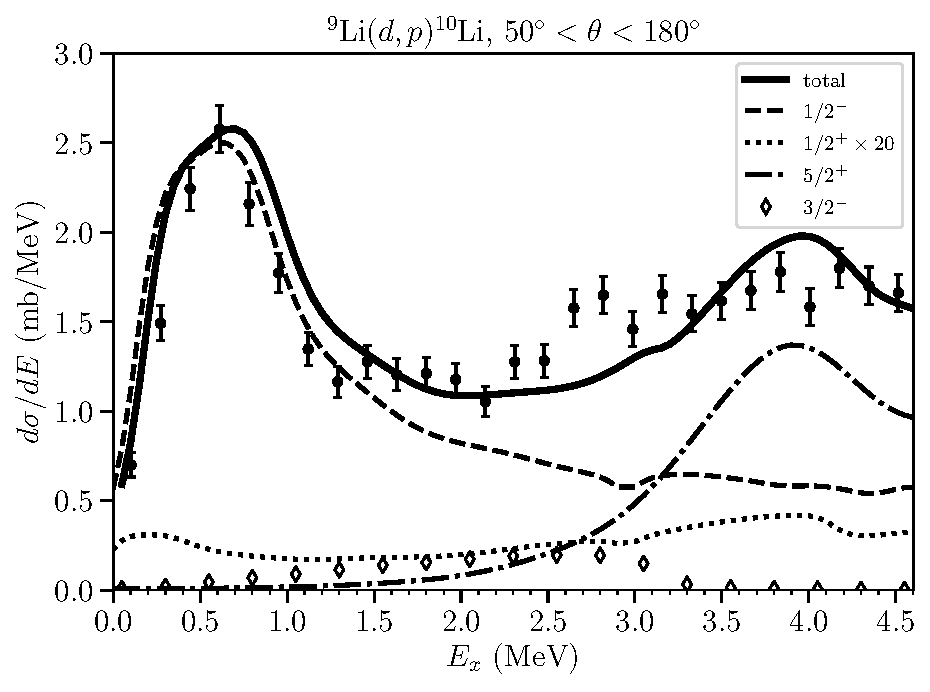
\includegraphics[width=12cm]{C6/figs_C6/FigBook1}}
	\caption{Theoretical predictions (continuous solid curve) of the $^{10}$Li strength function associated with the $^9$Li$(d,p)^{10}$Li reaction at 100 MeV incident energy at $5.5^\circ\leq\theta_{cm}\leq16.5^\circ$ in comparison with experimental data (solid dots with errors, \cite{Cavallaro:17}). The partial contributions are the incoherent sums of the strngth functions of the multiplets ($\widetilde {j}^\pi$, $1p_{3/2}(\pi)$). That is: (dashed line) $\widetilde j^\pi=\widetilde{1/2}^- (1^+,2^+)$; (dash-dotted line) $\widetilde{5/2}^+ (1^--4^-)$; (diamonds) $\widetilde{3/2}^- (0^+-3^+)$; (dotted line) $\widetilde{1/2}^+ (1^-,2^-)$ \textbf{multiplied by a factor of 20}.}\label{fig5.2.4}
\end{figure}
  \begin{figure}
	\centerline{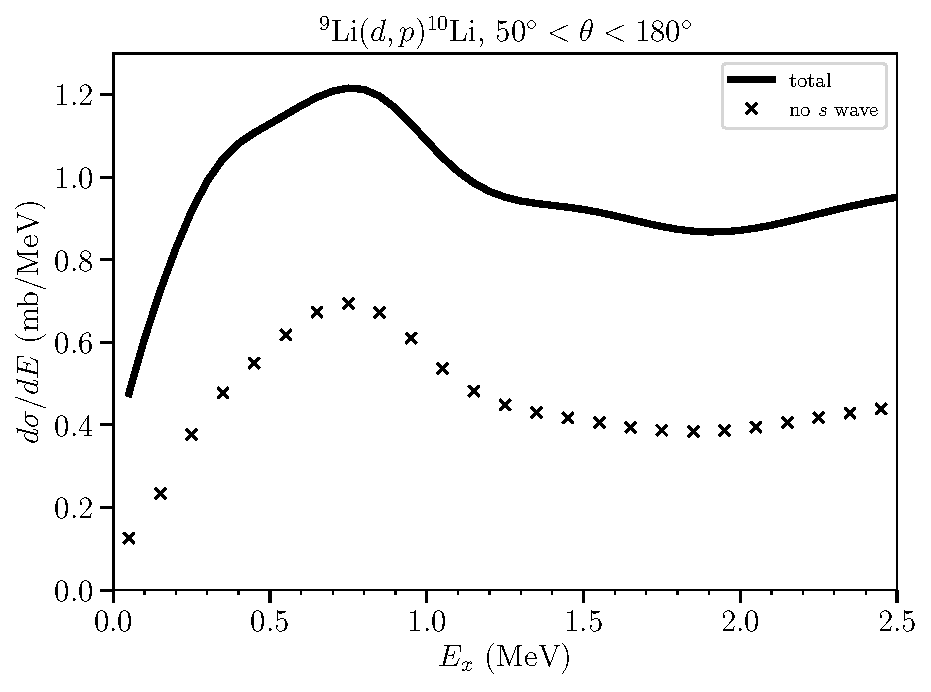
\includegraphics[width=12cm]{C6/figs_C6/FigBook3}}
	\caption{Predicted strength function obtained by integrating the absolute double differential cross section $d\sigma/dEd\Omega$ over the angular range $50^\circ\leq\theta_{cm}\leq180^\circ$.}\label{fig5.2.5}
\end{figure}
  \begin{figure}
	\centerline{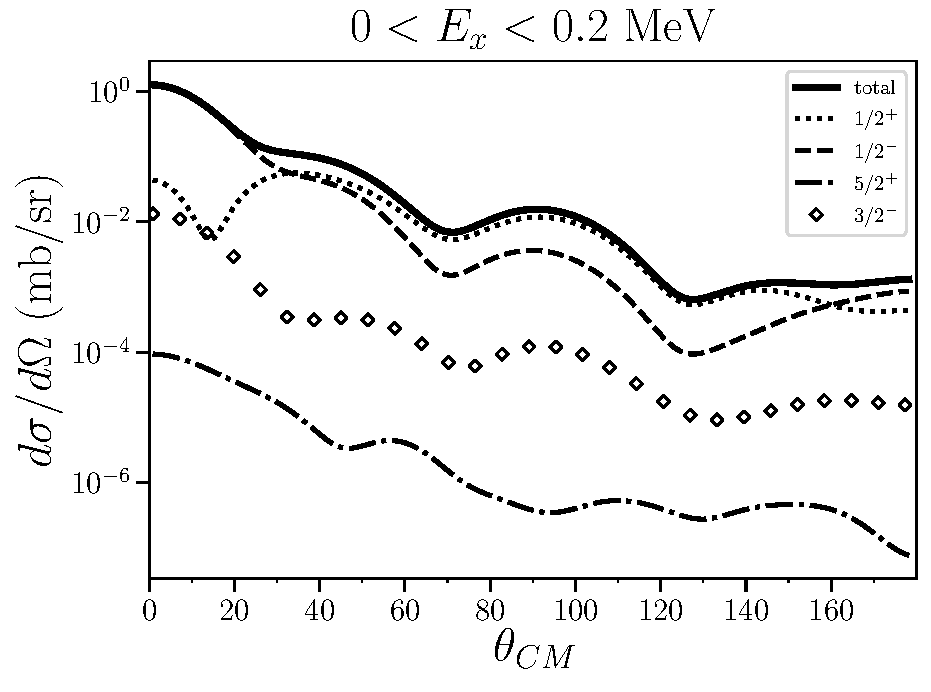
\includegraphics[width=12cm]{C6/figs_C6/FigBook2}}
	\caption{Predicted angular distributions ($d\sigma/d\Omega$) obtained by integrating the absolute double differential cross section $d\sigma/dEd\Omega$ in the energy interval 0--0.2 MeV. In the present case, and at variance with Fig. \ref{fig5.2.4}, no multiplicative factor was introduced in connection with $d\sigma_{\widetilde {1/2^+}}/d\Omega$.}\label{fig5.2.6}
\end{figure}

As seen from Fig. \ref{fig5.2.5} the situation changes radically if \textit{one puts the same question but changing the angular range from $5.5^\circ\leq\theta_{cm}\leq16.5^\circ$ into $50^\circ\leq\theta_{cm}\leq180^\circ$.} Equally univocally the answer now reads \textit{large}.

The reason at the basis of the essential difference between the two questions, and thus answers, is provided by the absolute differential cross section\footnote{The consistency with the $^9$Li$(d,p)^{10}$Li data of \cite{Jeppesen:06}, recorded in the angular range 98$^\circ\leq\theta_{cm}\leq134^\circ$ is apparent. For details see \cite{Barranco:20}. See also \cite{Moro:19}.} 
$d\sigma(\theta)_{\widetilde{1/2}^+}/d\Omega$ obtained integrating $d\sigma_{\widetilde{1/2}^+}/dEd\Omega$ over the energy interval 0--0.2 MeV. As observed from Fig. \ref{fig5.2.6} it results from a blend of structure, related to the single-particle content of the state (\ref{eq5.2.1}), and the interference pattern displayed by the outgoing distorted waves which displays a minimum close to $\theta_{cm}=16.5^\circ$. Returning to Fig. \ref{fig5.2.4}, and still within the above scenario, one can posit that the overall agreement between theory and experiment observed for $\left.d\sigma/dE\right)_{5^\circ-16.5^\circ}$ within the energy range 3--4.5 MeV provides quantitative, although indirect, evidence of the presence
of a robust $1/2^+$ state at low energy. This is in keeping with the strong coupling found in the NFT results between the $s_{1/2}$ and $d_{5/2}$ virtual and resonant states, through the quadrupole vibration of the core $^9$Li. In fact, due to this strong mixing either one reproduces both the $d\sigma_{\widetilde{1/2}^+}/dE$ and the $d\sigma_{\widetilde{5/2}^+}/dE$ strength functions or likely none of them\footnote{Within this context see \cite{Barranco:20}. See also \cite{Moro:19}.}. Because these couplings renormalize single-particle content, energies, and widths, as well as the radial dependence of the wavefunctions (form factors), all these elements have to be calculated self-consistently. The role played by such requirements is likely emphasized in the case like the present one, of continuous spectroscopy, in which structure and reaction are, in a very real sense, just two aspects of the same physics. 


Before concluding the present section, it may be useful to remind us what, within the framework of quantum mechanics, one can learn from a reaction experiment. It is not ``what is the state after the collision'' but ``how probable is a given effect of the collision''\footnote{\cite{Born:26}. If there is a lesson to be learned from the above discussion is the fact that, in dealing with a specific feature of a quantal many--body system, e.g. single-particle motion in nuclei (structure) and one-particle transfer process (reaction), one can hardly avoid to talk about other elementary modes of excitation and  reaction channels, respectively. Within the scenario of the chosen example, this is because a nucleon which, in first approximation is in a mean field stationary state, can actually be viewed as a fermion moving through a gas of  quadrupole phonons to which it couples, becoming eventually heavier because dressed by the phonons (case of $s_{1/2}$). But also,   because of Pauli principle the nucleon  is forced to exchange role with the nucleons of the composite (particle-hole) phonons undergoing repulsion (case of $p_{1/2}$).}.

\begin{subappendices}
\section[Minimal mean field theory]{Minimal requirements for a consistent mean field theory}\label{C6AppA}
As seen from Figs. \ref{fig1.0.6}--\ref{fig1.0.8}  the minimum requirements of selfconsistency to be imposed upon single-particle motion requires both non-locality in space (HF) and in time (TDHF)
\begin{equation}\label{eq6.A.1}
i\hbar \frac{\partial \varphi_\nu}{\partial t}=-\frac{\hbar^2}{2 m}\nabla^2 \varphi_\nu(x,t)+\int dx'dt'U(x-x',t-t')\varphi_\nu(x',t').
\end{equation}
 Assuming, for simplicity, infinite nuclear matter (confined by a constant potential of depth $V_0$), and thus plane wave solutions, the above time-dependent Schr\"{o}dinger equation leads to the quasiparticle dispersion relation 
\begin{equation}\label{eq6.A.2}
\hbar\omega=\frac{\hbar^2k^2}{2m^*}+\frac{m}{m^*}V_0,
\end{equation}
where the effective mass
\begin{equation}\label{eq4.A.3}
m^*=\frac{m_k m_\omega}{m},
\end{equation}
is the product of the $k$-mass
\begin{equation}
m_k=m\left(1+\frac{m}{\hbar^2k}\frac{\partial U}{\partial k}\right)^{-1},
\end{equation}
closely connected with the Pauli principle $\left(\frac{\partial U}{\partial k}\approx \frac{\partial U_x}{\partial k}\right)$, while the $\omega$--mass
\begin{equation}\label{eq6A5}
m_\omega=m\left(1-\frac{\partial U}{\partial \hbar \omega}\right),
\end{equation}
results from the dressing of the nucleon through the coupling with the (quasi) bosons. 
% \begin{figure}
%\centerline{\includegraphics*[width=10cm,angle=0]{C6/figs_C6/fig6_A1}}
%\caption{\textbf{(a)}  Scattering of two nucleons through the bare $NN$-interaction \mbox{$v|\mathbf{r}-\mathbf{r}'|$}, \textbf{(b)} contribution to the direct ($U$, Hartree) and \textbf{(c)} to the exchange ($U_x$, Fock) potential, resulting in \textbf{(d)} the (static) self-consistent relation between potential and density (non--local \textbf{(d')}), which \textbf{(e)} uncouples occupied ($\varepsilon_\nu\leq\varepsilon_F$) from empty states ($\varepsilon_\nu>\varepsilon_F$), \textbf{(f)} multiple scattering of two nucleons lead, through processes like the one depicted in \textbf{(g)}, eventually propagated to all orders, to: \textbf{(h)} softening of the discontinuity of the occupancy of levels at $\varepsilon_F$, as well as to: \textbf{(i)} generalization of the static selfconsistency into a dynamic relation encompassing also collective vibrations (Time-Dependent HF).}\label{fig6_A1}
%\end{figure}

 The occupancy of levels around $\varepsilon_F$ is related to $Z_\omega$, a quantity which measures the discontinuity at the Fermi energy  and which is equal to $m/m_\omega$.  This is in keeping with the fact that the time the nucleon is coupled to the vibrations it cannot behave as a single-particle and can thus not contribute to e.g. the single-particle pickup cross section. \textit{The particle-vibration coupling not only renormalizes energies and single-particle content but also the radial dependence of the wavefunction (formfactors).}

















It is of notice that the self-consistence requirements for the iterative solution of Eq. (\ref{eq6.A.1}) reminds very much those associated with the solution of the Kohn-Sham equations in finite systems,
 \begin{equation}
 H^{KS}\varphi_\gamma(\mathbf{r})=\lambda_\gamma\varphi_\gamma(\mathbf{r}),
 \end{equation}
where
 \begin{equation}
 H^{KS}=-\frac{\hbar^2}{2 m_e}\nabla^2+U_H(\mathbf{r})+V_{ext}(\mathbf{r})+U_{xc}(\mathbf{r}),
 \end{equation}
$H^{KS}$ being known as the Kohn-Sham Hamiltonian, $V_{ext}(\mathbf{r})$ being the field created by the ions and acting on the electrons. Both the Hartree and the exchange--correlation potentials $U_H(\mathbf{r})$ and $U_{xc}(\mathbf{r})$ depend on the (local) density, hence on the whole set of wavefunctions $\varphi_\gamma(\mathbf{r})$. Thus, the set of $KS$--equations must be solved selfconsistently\footnote{See e.g. \cite{Broglia:04b} and refs. therein.}.
\subsection{Density of levels}\label{C4AppA1}
Making use of Eq. (\ref{eq6.A.2})  ($E=\hbar\omega$), one can calculate $dE/dk$ for a single nucleon and one spin orientation\footnote{\cite{Mahaux:85}, p. 17.}. The inverse of this expression is\footnote{P. F. Bortignon, private communication.}
\begin{align}
\frac{dk}{dE}=\frac{m^*}{\hbar^2k},
\end{align} 
which testifies to the fact that the energy spacing between levels, i.e. the density of levels (see below), changes as $m^*$ does.

One can then calculate the average value over the Fermi distribution, obtaining
\begin{align}
\left\langle\frac{dk}{dE}\right\rangle=\frac{m^*}{\hbar^2(2/3)k_F}.
\end{align}
 Let us now take into account all nucleons, both spin orientations and eliminate the unit (inverse) length, i.e
\begin{align}
\frac{2A}{k_F}\left\langle\frac{dk}{dE}\right\rangle=3A\frac{m^*}{\hbar^2k_F^2}=3A\frac{m^*}{2m\epsilon_F}.
\end{align}
Assuming $m^*=m_\omega m_k/m\approx m$, where $m$ is the experimental nucleon mass one obtains
\begin{align}
\frac{3}{2}\frac{A}{\epsilon_F},
\end{align}
a value which coincides with the Fermi gas model estimate for the one--particle level density $g_0$\footnote{See e.g. \cite{Bohr:69} Eq. (2-48).}. Taking properly into account the geometry of the system, one obtains
\begin{align}\label{eq4A13}
a=\frac{\pi^2}{6}\frac{3}{2}\frac{A}{\epsilon_F}
\end{align}
for the prefactor of the exponential of the Fermi expression of the total density of single particle levels. Making use of $\epsilon_F=36$ MeV leads to,
\begin{align}\label{eq4A13x}
a\approx\frac{A}{14}\text{MeV}^{-1}.
\end{align}
In keeping with the fact that one can interpret $dE/dk$ as the rate of change in energy when the momentum changes or, equivalently, when the number of nodes per unit length changes, and this can be used to label the single--particle states, (\ref{eq4A13x}) can be confronted at profit with the average degeneracy per unit energy of valence orbitals (see Table \ref{tab4A1}). 



Within this context it is of notice that an estimate of the quantity $a$ based on the harmonic oscillator, leads to $a\approx\frac{\pi^2}{6}\frac{(N_{max}+3/2)^2}{\hbar\omega_0}$ i.e. an expression inversely proportional to the (constant) energy separation of levels \footnote{See \cite{Bohr:69} p. 188, Eq (2-125a).}. In an attempt to bridge the gap between the nuclear matter expressions discussed above and finite nuclei, i.e. potential wells of finite range, we consider
\begin{align}\label{eq4A14}
H=\frac{p^2}{2D}+\frac{C}{2}x^2,
\end{align}
$(p=D\dot x)$ which leads to a constant level spacing,
\begin{align}
\hbar\omega_0=\hbar\sqrt{\frac{C}{D}},
\end{align}
 and implies that the density of states is proportional to the square root of the particle inertia (mass). However, this result follows from the assumption that the potential remains unchanged if the bare mass (in which case $D$ is, for example, set equal to the HF $k$--mass, $m_k$) is replaced by an effective mass $m^*$ (e.g. $m_km_\omega/m$, Eq. (\ref{eq4.A.3})). In this case the ground state wavefunction
 
\begin{align}\label{eq4A15}
\varphi_0\sim\exp\left(-\frac{x^2}{2b^2}\right),
\end{align}
with,
\begin{align}\label{eq4A16}
b=\sqrt{\frac{\hbar}{m^*\omega_0}},
\end{align}
for a dressed nucleon of effective mass $m^*>D$ will shrink in space compared with the one of mass $D$ and consequently the mean square radius of the system
\begin{align}\label{eq4A17}
\left\langle r^2\right\rangle=\frac{\hbar}{m^*\omega_0}\left(N+\frac{3}{2}\right)=b^2\left(N+\frac{3}{2}\right)
\end{align}
will decrease. This is not correct, and one has to impose the condition $b^2$=constant. A condition which implies that the energy difference between levels is inversely proportional to the effective mass of the nucleon\footnote{See Sect. \ref{S3.2}, Eq. (\ref{eq2_2_2}); also Fig. \ref{figintro6} inset (c).}, that is,
\begin{align}\label{eq4A18x}
\hbar\omega_0=\frac{\hbar^2}{m^*b^2}.
\end{align}
Let us conclude this Appendix with a remark concerning the dimensions of the parameters $D$ and $C$ entering Eq. (\ref{eq4A14}). Because the variable $x$ has dimensions of length ($[x]$=fm), the dimensions of the inertia and restoring force parameters are

\begin{align*}
[C]=\text{MeV fm}^{-2}\quad\text{and}\quad [D]=\text{MeV fm}^{-2}\text{s}^2.
\end{align*}
Consequently the associated zero point fluctuations
\begin{align}\label{eq4A18}
\sqrt{\frac{\hbar\omega_0}{2C}}=\sqrt{\frac{\hbar^2}{2D}\frac{1}{\hbar\omega_0}}
\end{align}
have dimensions of fm. It is of notice that in the case of the harmonic oscillator Hamiltonian (\ref{eq1.0.7}), the associated ZPF is a $c$-number, in keeping with the fact that the (dynamic) deformation parameter $\alpha$ is dimensionless and thus $[D]$=MeV$s^2$ and [$C$]=MeV. 
    \begin{table}
    \centering
    \begin{tabular}{|c|c|c|}
\hline
&\multicolumn{2}{c|}{MeV$^{-1}$}\\
\cline{2-3}
&empirical& $a$\\
\hline
$^{208}_{82}$Pb$_{126}$& 17($10^{a)}+7^{b)}$)& 15($9^{a)}+6^{b)}$)\\
\hline
$^{120}_{50}$Sn$_{126}$& 4$^{a)}$& 5$^{a)}$\\
\hline
    \end{tabular}\\$a)$ neutrons\\$b)$ protons\\\caption{
    Comparison of the factor (\ref{eq4A13x}) ($a=n/14$MeV$^{-1}$) corresponding to $^{208}$Pb for both $n=N$ and $n=Z$ and for $^{120}$Sn in the case of $n=N$, in comparison with the empirical value associated with the valence orbitals of these nuclei. That is $(h_{9/2},f_{7/2},i_{13/2},p_{3/2},f_{5/2},p_{1/2},g_{9/2},i_{11/2},d_{5/2},j_{15/2},s_{1/2},g_{7/2},d_{3/2})$ and $(g_{7/2},d_{5/2},h_{11/2},d_{3/2},s_{1/2},h_{9/2},f_{7/2},i_{13/2})$ for neutrons and protons in $^{208}$Pb, leading to $\sum_j^N(2j+1)/\Delta E_N=102/10$ MeV$=10$ MeV$^{-1}$ and $\sum_j^Z(2j+1)/\Delta E_Z=64/(9$ MeV)$\approx7$ MeV$^{-1}$, where $\Delta E_N$ is the experimental energy interval over which the valence orbitals are distributed (see e.g. \cite{Bohr:69} p. 325, Fig. 3-3). In the case of neutrons of $^{120}$Sn, use is made of the dressed valence orbitals $d_{5/2},g_{7/2},s_{1/2},d_{3/2},h_{11/2}$ resulting from the renormalization of HF-Sly4 levels through the coupling of collective modes making use of nuclear field theory plus Nambu-Gorkov techniques ((NFT)+(NG); for details see \cite{Idini:15} and Table I of \cite{Potel:17}). The result, taking into account the breaking of the single--particle strength, in particular that of the $d_{5/2}$ orbital is $\sum_j^N(2j+1)/\Delta E_N=32/8$ MeV$\approx4$ MeV$^{-1}$.}\label{tab4A1}
    \end{table}
\section[Single-particle strength function]{Model for single--particle strength function:
 Dyson equation}\label{C6AppB}
In the previous Appendix we schematically introduced  arguments regarding the complexity of defining a ``bona fide'' single-particle spectroscopic factor. It was done with the help of Feynman (NFT) diagrams. In what follows we essentially repeat the arguments, but this time in terms of Dyson's (Schwinger) language.
 \begin{figure}
\centerline{\includegraphics*[width=10cm,angle=0]{C6/figs_C6/fig6_B1}}
\caption{Two state schematic model describing the breaking of the strength of the pure single--particle state $|a\rangle$, through the coupling to collective vibrations (wavy line) associated with polarization (PO) and correlation (CO) processes.}\label{fig6_B1}
\end{figure}
For simplicity, we consider a two--level model where the pure single--particle state $|a\rangle$ couples to a more complicated  (doorway) state
$|\alpha\rangle$, made out of a fermion (particle or hole), coupled to a particle--hole excitation which, if iterated to all orders can give rise to a collective state (Fig.\ref{fig6_B1}). The Hamiltonian describing the system is\footnote{ \cite{Bohr:69}.}
 \begin{equation}
 H=H_0+v,
 \end{equation}
 where
  \begin{equation}
  H_0|a\rangle=E_a|a\rangle,
  \end{equation}
  and
    \begin{equation}
    H_0|\alpha\rangle=E_\alpha|\alpha\rangle.
    \end{equation}
  Let us call $\langle a|v|\alpha\rangle=v_{a\alpha}$ and assume $\langle a|v|a\rangle=\langle \alpha|v|\alpha \rangle=0$.
  
  From the secular equation
\begin{equation}
\left(
\begin{matrix}
E_\alpha-E_i & v_{a\alpha}\\  
v_{a \alpha} & E_a-E_i \\ 
\end{matrix}
\right)
\left(
\begin{matrix}
C_\alpha(i)\\  
C_a(i)\\ 
\end{matrix}
\right)=0,
\end{equation}
and associated normalization condition
\begin{equation}\label{eqAp6B5}
C_a^2(i)+C_\alpha^2(i)=0,
 \end{equation}
one obtains
\begin{equation}\label{eqAp6B6}
C_a^2(i)=\left(1+\frac{v_{a\alpha}^2}{(E_\alpha-E_i)^2}\right)^{-1},
 \end{equation}
and 
\begin{equation}\label{eqAp6B7}
\Delta E_a(E)=E_a-E=\frac{v_{a\alpha}^2}{E_a-E}.
 \end{equation}
The energy of the correlated state
\begin{equation}\label{eqAp6B8}
|\tilde a\rangle=C_a(i)| a\rangle+C_\alpha (i)| \alpha\rangle,
 \end{equation}
is obtained by the (iterative) solution of the Dyson equation (\ref{eqAp6B7}), which propagate the diagrams shown in Figs \ref{fig6_B1} (a) and (b) to infinite order leading to collective vibrations (see Fig. \ref{fig6_B1} (c)).

With the help of the definition given in Eq. (\ref{eq6A5}), and making use of the fact that in the present case, the quantity $U$ appearing in this equation coincides, within the present context with $\Delta E_a(E)$, one obtains that the discontinuity of the single--particle levels at the Fermi energy is given by
\begin{equation}\label{eqAp6B4}
Z_\omega=C_a^2(i)=\left(\frac{m_\omega}{m}\right)^{-1}.
 \end{equation}
 Making use of the solution of  the Dyson equation (\ref{eqAp6B7}), and of the relations (\ref{eqAp6B5}) and (\ref{eqAp6B6}), one can calculate the renormalized state $|\tilde a\rangle$ (Eq. \ref{eqAp6B8}) to be employed in working out the associated, modified, single--particle transfer form factor needed in the calculation of the absolute value of one--particle transfer cross sections (cf. e.g. Sect. \ref{C6S2.1}, where the  above concepts and techniques are applied to the study of one-neutron transfer reactions in open shell, superfluid nucleus ($^{120}$Sn)).	 
 
\section[Vacuum and medium polarization]{Antiparticles: proof of concept of the quantal vacuum and of medium polarization effects}\label{C6AppCx}
 \begin{figure}
\centerline{\includegraphics*[width=13cm,angle=0]{C6/figs_C6/fig6_C1x}}
\caption{Feynman diagrams renormalizing the properties of a fermion.}\label{fig6_C1x}
\end{figure}
 \begin{figure}
	\centerline{\includegraphics*[width=15cm,angle=0]{C6/figs_C6/fig6_C2x}}
\caption{QED vacuum fluctuation (ZPF). In presence of e.g. an 	hydrogen atom (H), its electron is forced by Pauli principle to exchange with that of the ZPF, leading to a  CO (correlation) like process. Time ordering leads to PO (polarization) processes.}\label{fig6_C2x}
\end{figure}
 \begin{figure}
\centerline{\includegraphics*[width=10cm,angle=0]{C6/figs_C6/fig6_C3x}}
\caption{Lowest order diagrams which dress collective nuclear vibrations and GR.}\label{fig6_C3x}
\end{figure}

Let us consider a massive quantal particle, e.g., an electron, which moves at a velocity close of that of light. Because of Heisenberg relations, there exists a finite possibility to observe the particle moving at a velocity larger than its average velocity, and thus faster than light, a possibility ruled out by special relativity. To avoid this, one can introduce antiparticles, that is a hole in the ``vacuum'' filled to the rim (Fermi energy) with particles, thus providing the physics to the negative energy solutions of Dirac equation\footnote{See \cite{Klein:29}; see also \cite{Calogeracos:99}.}.

In other words, when an electron approaches the maximum speed with which information propagates in a medium, like e.g. in the case of an electron in the QED vacuum, processes like the one depicted in Fig. \ref{fig6_C1x} become operative. In other words, one can take care of the position indeterminacy of a quantal particle (electron) accepting the possibility to observe it through specific measurements which unavoidably create different particles, each of them identical to the original one, but with different positions, to keep track of conserved quantum numbers, these particles are to be accompanied by an equal number of antiparticles (positrons).

Similar results can be obtained by considering vacuum fluctuations (ZPF), and forcing them to become real through e.g. the Pauli principle  as observed in the Lamb shift (Fig. \ref{fig6_C2x}, cf. also Fig. \ref{fig6.2.1x}).


In the nuclear case the medium can, due to spatial quantization typical of Finite Quantal Many-Body Systems (FQMBS), propagate information with varied frequency. Typically, of few MeV (low-lying collective quadrupole and octupole vibrations to which one has to add  pygmy and allowing for high energy modes, also giant resonances, thus leading  to a rich number of CO and PO processes. This is in keeping with the fact that the intermediate boson (photon QED, vibrations of nuclear medium) propagates in a medium which is not isotropic, thus undergoing fragmentation of the associated strength (inhomogeneous damping, Fig. \ref{fig6_C3x}). To make even richer the nuclear scenario, collisional damping plays also a role in the strength function of giant resonances (GR). Nonetheless, the associated widths (lifetimes) are controlled by the coupling to doorway states (($2p-2h$) intermediate states built out of uncorrelated $p-h$ excitations and of a collective vibration), even at nuclear temperatures of 1--2 MeV, let alone when the GR is based on the ground state\footnote{Fig. \ref{fig6_C3x}; cf. \cite{Bortignon:98} and refs. therein, cf. also \cite{Broglia:87}.}. The strong cancellation found between self-energy and vertex correction diagrams, testify to the collectivity of nuclear vibrations (generalized Ward identities), and reminds of Furry's theorem (no coupling between one- and two-photon states or, more generally, diagrams containing loops with an odd number of quanta in it, are zero\footnote{See e.g. \cite{Mehra:96} p 264.}).
%
%\section{The Lamb Shift}\label{C6AppC}
% \begin{figure}
%\centerline{\includegraphics*[width=10cm,angle=0]{C6/figs_C6/fig6_C3}}
%\caption{Schematic representation of the processes associated with the Lamb shift.}\label{fig6_C1}
%\end{figure}
%In Fig. \ref{fig6_C1} we display a schematic summary of the electron--photon processes, associated with Pauli principle corrections, leading to the splitting of the lowest $s,p$ states of the hydrogen atom known as the Lamb shift\footnote{\cite{Lamb:47,Kroll:49}.}.
%
%
%In the upper part of the figure the predicted position of the electronic single--particle levels of the hydrogen atom as resulting from the solution of the Scr\"{o}dinger equation (Coulomb field). In the lowest part of the figure one displays the electron of an hydrogen atom (upwards going arrowed line) in presence of vacuum ZPF (electron--positron pair plus photon, oyster--like diagram).  Because the associated electron virtually occupies states already occupied by the hydrogen's electron, thus violating Pauli principle, one has to antisymmetrize the corresponding two-electron state. Such process gives rise to the exchange of the  fermionic lines and thus to CO-like diagrams. Also, through time ordering, to PO-like diagrams. The results provide a quantitative account of the experimental findings (see also Fig. \ref{fig6.2.1x}).  
\section{Self-energy and vertex corrections}\label{C6AppD}
 \begin{figure}
\centerline{\includegraphics*[width=10cm,angle=0]{C6/figs_C6/fig6_C1}}
\caption{Self energy (effective-mass-like) processes. The result of the probing with an external field (dotted line started with a cross, observer) of the properties (mass, charge, single-particle content, etc) of a fermion (e.g. an electron or a nucleon, arrowed line) dressed through the coupling to  bosons (photons or collective vibrations, wavy line), results from the modulus squared of the sum of the amplitudes associated with each of the four diagrams (a)--(d) (cf. \citep{Feynman:75}).}\label{fig6_D1}
\end{figure}
 \begin{figure}
\centerline{\includegraphics*[width=10cm,angle=0]{C6/figs_C6/fig6_C2}}
\caption{(a), (b) Vertex corrections. These are triple-interaction  diagrams (phonon, particle and hole lines) in which none of the incoming lines can be detached from either of the other two by cutting one line. In connection with condensed matter Migdal's theorem  (\cite{Migdal:58}) states that for phonons, (\cite{Bardeen:55},  \cite{Frohlich:52}) vertex corrections can be neglected (cf. also \cite{Anderson:64}). Vertex corrections are, as a rule, important in the nuclear case where they lead to conspicuous cancellations of the self-energy contributions (d) and (e) (cf. e.g. \cite{Bortignon:83}, cf. also \cite{Anderson:64}). The solid grey circle in (c) represents the effective, renormalized vertex. }\label{fig6_D2}
\end{figure}
In Fig. \ref{fig6_D1} an example of the fact that in field theories (e.g. QED or NFT), nothing is really free and that e.g., the bare mass of a fermion (electron or nucleon), is the parameter one adjusts so that the renormalized particle displays properties which agree with experimental findings, for example the observed mass (single particle energy). In Fig. \ref{fig6_D2}, lowest order diagrams associated with the renormalization of the fermion--boson interaction (vertex corrections) are given. The sum of contributions (a) and (b) can, in principle, be represented by a renormalized vertex (see. diagram (c)). There is, as a rule, conspicuous interference (e.g. cancellation) in the nuclear case between vertex and self-energy contributions (see diagrams (a) and (d)+(e) of Fig. \ref{fig6_D2}, a phenomenon closely related with conservation laws\footnote{ \cite{Schrieffer:64}); see also Fig. \ref{fig6_C3x} and refs. \cite{Bortignon:81,Bertsch:83} and \cite{Bortignon:98} pp. 82--86.}. In particular, cancellation in the case in which the bosonic modes are of isoscalar character\footnote{\cite{Bortignon:83}.}. Consequently, one has to sum explicitly the different amplitudes with the corresponding phases and eventually take the modulus squared of the result to eventually obtain the quantities to be compared with the data, a fact that call attention to the use of an effective, $\omega$-independent (renormalized) vertex.

Within the framework of QED the above mentioned cancellations are exact implying that the interaction between one- and two-photon states vanishes (Furry theorem). The physics at the basis of the cancellation found in the nuclear case can be exemplified by looking at a spherical nucleus displaying a low-lying collective quadrupole vibration. The associated zero point fluctuations (ZPF) lead to time dependent shapes with varied instantaneous values of the quadrupole moment. In other words, a component of the ground state wavefunction ($|(j_p \otimes j_h^{-1})_{2^+} \otimes 2^+; 0^+\rangle $), which can be viewed as a  gas of quadrupole (quasi) bosons promoting a nucleon across the Fermi energy (particle-hole excitation) will lead to fermionic states which behave as having a positive (particle) and a negative (hole) effective quadrupole moment, in keeping with the fact that the closed shell system is spherical, and thus has zero quadrupole moment. 

\section{Single-nucleon transfer for pedestrians}\label{C6AppE}

In what follows we discuss some aspects of the relations existing between nuclear structure and one-particle transfer cross sections. To do so, we repeat some of the steps carried out in Sect. \ref{C4S1}, but this time in a simpler and straightforward way, ignoring the complications associated with the spin carried out by the particles, the spin-orbit dependence of the optical model potential, the recoil effect, etc.

We consider the case of $A(d,p)A+1$ reaction, namely that of neutron stripping. The intrinsic wave functions $\psi_\alpha$ and $\psi_\beta$, where $\alpha=(A,d)$ and $\beta=((A+1),p)$,
\begin{subequations}
\begin{align}\label{eqC6E1}
&\psi_\alpha=\psi_{M_{A}}^{I_A}(\xi_A) \phi_d(\vec r_{np}),\\
\begin{split}\label{eqC6E1b}
&\psi_\beta=\psi_{M_{A+1}}^{I_{A+1}}(\xi_{A+1})\\
& \;\;\;\;=\sum_{l,I'_A} (I'_A;l \vert \} I_{A+1})
[\psi^{I'_A}(\xi_A)\phi^l(\vec r_{n})]_{M_{A+1}-M_A}^{I_{A+1}},
\end{split}
\end{align}
\end{subequations}
where $(I'_A;l \vert \} I_{A+1})$ is a generalized fractional parentage coefficient. It is of notice that, as a rule,  \mbox{$(I'_A;l \vert \} I_{A+1})\,\phi^l(\vec r_{n})$} should be able to describe a dressed quasiparticle state containing only a fraction of the  single particle strength. Although ignoring possible radial renormalization we assume, for simplicity, the expansion to be operative.	
To further simplify the derivation we assume we are dealing with spinless particles. This is the reason why no ``intrinsic'' proton wavefunction appears in Eq. (\ref{eqC6E1b}). The variable $\vec r_{np}$ is the relative coordinate of the proton and the neutron (see Fig. \ref{fig6_E1}).


The transition matrix element can now be written as
\begin{equation}\label{eq423}
 \begin{split}
T_{d,p}&= \langle \psi_{M_{A+1}}^{I_{A+1}}(\xi_{A+1}) \chi^{(-)}_p(k_p,\vec{r}_p),
V'_\beta \, \psi_{M_{A}}^{I_{A}}(\xi_{A}) \chi^{(+)}_d(k_d,\vec{r}_d)\rangle \\
&= \sum_{\substack{l,I'_A\\M'_A}} (I'_A;l \vert \} I_{A+1}) (I'_A \,M'_A\, l\, M_{A+1}-M'\,_A \vert I_{A+1}\,M_{A+1})\\
& \times\int d\vec{r}_n d \vec{r}_p \chi^{* (-)}_p(k_p,\vec{r}_p) \phi_{M_{A+1}-M'_A}^{*l}(\vec{r}_n)
(\psi_{M_{A}}^{I_{A}}(\xi_{A}),V'_\beta \psi_{M'_{A}}^{I'_{A}}(\xi_{A}))\\
& \times\phi_d(\vec r_{np})
\chi^{(+)}_d(k_d,\vec{r}_d) \; \delta_{I'_A,I_A} \; \delta_{M'_A,M_A}.
\end{split}
\end{equation}
In the stripping approximation
\begin{equation}\label{eq424}
 \begin{split}
V'_\beta & = V_\beta(\xi,\vec r_\beta)- \bar U_\beta (r_\beta)\\
&=V_\beta(\xi_A,\vec r_{pA})+V_\beta(\vec r_{pn})-\bar U_\beta (r_{pA}).
\end{split}
\end{equation}
Then
\begin{equation}\label{eq425}
 \begin{split}
(\psi_{M_{A}}^{I_{A}}(\xi_{A}) & ,V'_\beta \psi_{M_{A}}^{I_{A}}(\xi_{A}))=
(\psi_{M_{A}}^{I_{A}}(\xi_{A}), V_\beta(\xi_A,\vec r_{pA}) \psi_{M_{A}}^{I_{A}}(\xi_{A}))\\
&+(\psi_{M_{A}}^{I_{A}}(\xi_{A}), V_\beta(\vec r_{pn})
\psi_{M_{A}}^{I_{A}}(\xi_{A}))- \bar U_\beta (r_{pA}).
\end{split}
\end{equation}
We assume
\begin{equation}\label{eq426}
  U_\beta (r_{pA})=(\psi_{M_{A}}^{I_{A}}(\xi_{A}), V_\beta(\xi_A,\vec r_{pA}) \psi_{M_{A}}^{I_{A}}(\xi_{A})).
\end{equation}
Then
\begin{equation}\label{eq427}
(\psi_{M_{A}}^{I_{A}}(\xi_{A}), V'_\beta\, \psi_{M_{A}}^{I_{A}}(\xi_{A}))= V_{np}(\vec r_{pn}).
\end{equation}
 \begin{figure}
\centerline{\includegraphics*[width=7cm,angle=0]{C6/figs_C6/fig6_E1}}
\caption{Coordinates used in the description of the $A (d,p)(A+1)$ stripping process.}\label{fig6_E1}
\end{figure}

Inserting eq. (\ref{eq427}) into eq. (\ref{eq423}) we obtain
 \begin{equation}\label{eq428}
 \begin{split}
T_{d,p}&= \sum_l (I_A;l \vert \} I_{A+1}) (I_A\, M_A\, l\, M_{A+1}-M_A \vert I_{A+1}\,M_{A+1})  \\
&\times\int d\vec{r}_n d \vec{r}_p \chi^{* (-)}_p(k_p,\vec{r}_p) \phi_{M_{A+1}-M_A}^{*l}(\vec{r}_n)
V(\vec r_{pn}) \phi_d(\vec r_{np})
\chi^{(+)}_d(k_d,\vec{r}_d)
\end{split}
\end{equation}
The differential cross section is then equal to
\begin{equation}\label{eq429}
\frac{d \sigma}{d \Omega} = \frac{2}{3} \frac{\mu_p \mu_d}{(2\pi \hbar^2)^2}\frac{(2I_{A+1}+1)}{(2I_A+1)}
\frac{k_p}{k_d}\sum_{l,m_l}\frac{(I_A;l \vert \} I_{A+1})^2}{2l+1} \vert B_{m_l}^l\vert ^2,
\end{equation}
where
\begin{equation}\label{eq430}
B_{m_l}^l(\theta)=\int d\vec{r}_n d \vec{r}_p \chi^{* (-)}_p(k_p,\vec{r}_p) Y_m^{*l}(\hat r_n) u_{nl}(r_n)
V(\vec r_{pn}) \phi_d(\vec r_{np})
\chi^{(+)}_d(k_d,\vec{r}_d)
\end{equation}
and
\begin{equation}\label{eqC6E10}
\phi_m^{l}(\vec{r}_n)=u_{nl}(r_n) Y_m^{l}(\hat r_n),
\end{equation}
is the single-particle wave function of a neutron bound to  the core A. For simplicity, the radial wave function $u_{nl}(r_n)$ can be assumed to be a solution of a Saxon-Woods potential of parameters $V_0\approx 50$ MeV, $a=0.65$ fm and $r_0=1.25$ fm.



The relation (\ref{eq429}) gives the cross section for the stripping from the projectile of a neutron that would correspond to the n$^{\mathrm{th}}$ valence neutron in the nucleus ($A+1$). If we now want the cross section for stripping any of the valence nutrons of the final nucleus from the projectile, we must multiply eq. (\ref{eq429}) by $n$. A more careful treatment of the antisymmetry with respect to the neutrons shows this to be the correct answer.


Finally we get
\begin{equation}\label{eq432}
\frac{d \sigma}{d \Omega}=\frac{(2I_{A+1}+1)}{(2I_A+1)} \sum_l S_l \sigma_l(\theta),
\end{equation}
where
\begin{equation}\label{eq433}
S_l= n (I_A;l \vert \} I_{A+1})^2,
\end{equation}
and
\begin{equation}\label{eq434}
\sigma_l(\theta)=\frac{2}{3} \frac{\mu_p \mu_d}{(2\pi \hbar^2)^2}
\frac{k_p}{k_d}\frac{1}{2l+1}\sum_{m} \vert B_{m}^l\vert^2
\end{equation}


The distorted wave softwares evaluate numerically  the quantity $B_{m_l}^l(\theta)$, using for the wave functions $\chi^{(-)}$ and $\chi^{(+)}$ the solution of the optical potentials that fit the elastic scattering, i.e.
\begin{equation}\label{eq435}
(-\nabla ^2+\bar U-k^2) \chi=0,
\end{equation}
Note that if the target nucleus is even--even, $I_A=0$,  $l=I_{A+1}$. That is, only one $l$ value contributes in Eq. (\ref{eq429}), and the angular distribution is uniquely given by $\sum_{m} \vert B_{m}^l\vert^2$. The $l$-dependence of the angular distributions helps to identify $l=I_{A+1}$. The factor $S_l$ needed to normalize the calculated function to the data yields (assuming a good fit to the angular distribution), is known in the literature as the spectroscopic factor. It was assumed in the early stages of studies of nuclear structure with one--particle transfer reactions not only that it could be defined, but also that it contained all the nuclear structure information (aside from that associated with the angular distribution) which could be extracted from single--particle transfer. In other words, that it was the bridge directly connecting theory with experiment. \emph{Because nucleons are never bare, but are dressed by the coupling to collective modes, coupling which renormalizes not only the single-particle content but also the single-particle wavefunctions (formfactors),   the spectroscopic factor approximation is at best a helpful tool to get order of magnitude information from one--particle transfer data}.



There is a fundamental problem which makes the handling of integrals like that of (\ref{eq430}) difficult to handle, if not numerically at least conceptually. This difficulty is connected with the so called recoil effect \footnote{While this effect could be treated in a cavalier fashion in the case of light ion reactions ($m_a/m_A\ll 1$), this was not possible in the case of heavy ion reactions, as the change in momenta involved was always sizeable (cf. \citet{Broglia:04a} and refs. therein).}, namely the fact that the center of mass of the two interacting particles in entrance ($\mathbf r_{\alpha}: \alpha=a+A$) and exit  ($\mathbf r_{\beta}: \beta=b+B$) channels is different. This is at variance with what one is accustomed to deal with in nuclear structure calculations, in which the Hartree potential depends on a single coordinate, as well as in the case of elastic and inelastic reactions, situations in which $\mathbf r_{\alpha}=\mathbf r_{\beta}$. When $\mathbf r_{\alpha}\neq\mathbf r_{\beta}$ we enter a rather more complex many--body problem, in particular if continuum states are to be considered, than nuclear structure practitioners were accustomed to.
 
 
 Of notice that similar difficulties have been faced in connection with the non--local Fock (exchange) potential. As a rule, the corresponding (HF) mean field equations are rendered local making use of the $k$--mass approximation or within the framework of Local Density Functional Theory (DFT), in particular with the help of the Kohn--Sham equations\footnote{\cite{Mahaux:85}, \cite{Broglia:04b} and refs. therein; see also App. \ref{C6AppA}.}. Although much of the work in this field is connected with the correlation potential  (interweaving of single--particle and collective motion), an important fraction is connected with the exchange potential.
 
 
 In any case, and returning to the subject of the present appendix, it is always useful to be able to introduce approximations which can help the physics which is at the basis of the phenomenon under discussion (single--particle motion) emerge in a natural way, if not to compare in detail with the experimental data. 
Within this context, to reduce the integral (\ref{eq430}) one can assume that the proton-neutron interaction $V_{np}$ has zero-range, i.e.
\begin{equation}\label{eqC6AppE15}
 V_{np}(\vec r_{np})\phi_d(\vec r_{np})=D_0 \delta(\vec r_{np})
\end{equation}
so that  $B_{m}^l$ becomes equal to
\begin{equation}\label{eqC6E16}
B_{m_l}^l(\theta)=D_0 \int d\vec r \chi^{* (-)}_p(k_p,\vec r) Y_{m_l}^{*l}(\hat r) u_{l}(r)
\chi^{(+)}_d(k_d,\vec r),
\end{equation}
which is  a three dimensional integral, but in fact essentially a one--dimensional integral, as the integration over the angles can be worked out analytically.


\subsection{Plane-wave limit}


If in Eq. (\ref{eq435}) one sets $\bar U=0$, the distorted waves become plane waves i.e.
 \begin{subequations}
\begin{align}\label{eq437}
&\chi^{(+)}_d(k_d,\vec r)=e^{i \vec k_d \cdot \vec r},\\
&\chi^{*(-)}_d(k_p,\vec r)=e^{-i \vec k_p \cdot \vec r}.
\end{align}
\end{subequations}
Equation (\ref{eqC6E16}) can now be written as
\begin{equation}\label{eq438}
B_{m}^l=D_0 \int d\vec r e^{i (\vec k_d-\vec k_p) \cdot \vec r} Y_m^{*l}(\hat r) u_{l}(r).
\end{equation}
The linear momentum transferred to the nucleus is $\vec k_d-\vec k_p=\vec q$.
Let us expand $e^{i \vec q \cdot \vec r}$ in spherical harmonics, i.e.
\begin{equation}\label{eq439}
\begin{split}
 e^{i \vec q \cdot \vec r}&=\sum_l i^l j_l(qr)(2l+1)P_l(\hat q \cdot \hat r)\\
& =4 \pi \sum_l i^l j_l(qr)\sum_m Y_m^{*l}(\hat q) Y_m^{l}(\hat r),
\end{split}
\end{equation}
so
\begin{equation}\label{eq440}
 \int d\hat r e^{i \vec q \cdot \vec r} Y_m^{l}(\hat r)= 4 \pi i^l j_l(qr) Y_m^{*l}(\hat q).
\end{equation}
Then
\begin{equation}\label{eq441}
\begin{split}
 \sum_{m} \vert B_{m}^l\vert^2 & = \sum_{m} \vert Y_m^{l}(\hat q)\vert^2 D_0^2 16 \pi^2 \times \\
& \left \vert \int r^2 dr j_l(qr) u_l(r) \right \vert ^2=\\
& \frac{2l+1}{4 \pi} D_0^2 16 \pi^2 \left \vert \int r^2 dr j_l(qr) u_l(r) \right \vert ^2.
\end{split}
\end{equation}
Thus, the angular distribution is given by the integral $\left \vert \int r^2 dr j_l(qr) u_l(r) \right \vert ^2$. If one assumes that the process takes place mostly on the surface, the angular distribution will be given by $ \vert j_l(qR_0) \vert ^2$, where $R_0$ is the nuclear radius.

\begin{figure}
\centerline{\includegraphics*[width=15cm,angle=0]{C6/figs_C6/fig6_F2}}
\caption{Plane wave approximation analysis of three $^{44}$Ca(d,p)$^{45}$Ca differential cross sections leading to the ground state ($l_n=3$) and to the 1.9 MeV state ($l_n=1$) and 2.4 MeV ($l_n=0$) excited states, i.e.  $f_{9/2}$, $p_{1/2}$ and $s_{1/2}$ states \citep{Cobb:57}.}\label{fig3}
\end{figure}

We then have
\begin{equation}\label{eq442}
 \begin{split}
  q^2&= k_d^2+k_p^2- 2 k_d k_p \cos(\theta)\\
& =(k_d^2+k_p^2- 2 k_d k_p) + 2 k_d k_p (1-\cos(\theta))\\
& =(k_d-k_p)^2+ 4 k_d k_p \left(\sin (\theta/2)\right) ^2  \\
& \approx 4 k_d k_p \left(\sin (\theta/2)\right) ^2,
\end{split}
\end{equation}
since $ k_d \approx k_p $ for stripping reactions at typical energies. Thus the angular distribution has a diffraction-like structure given by
\begin{equation}\label{eq443}
\vert j_l(qR_0) \vert ^2= j_l^2 (2R_0 \sqrt{k_d k_p} \sin (\theta/2)).
\end{equation}
The function $j_l(x)$ has its first maximum at $x=l$, i.e. where
\begin{equation}\label{eq444}
\sin (\theta/2)=\frac{l}{2 R_0 k},\quad \quad (k_p \approx  k_d=k),
\end{equation}
Examples of the above relation are provided in Fig. \ref{fig3}.

\section{One--particle knockout within DWBA}\label{C6AppF}
\subsection{Spinless particles}
We are going to consider the reaction $A+a \rightarrow a+b+c$, in which the cluster $b$ is knocked out from the nucleus $A(=c+b)$. Cluster $b$ is thus initially bound, while the final states of $a,b$ and the initial state of $a$ are all in the continuum, and can be described with distorted waves defined as scattering solutions of an optical potential. A schematic depiction of the situation is shown in Fig. \ref{figC6F1}. While the derivation presented below is quite general, special emphasis is set to one--particle knock--out processes. 
\subsubsection{Transition amplitude}
A first derivation will be given in which, for simplicity, all the ``particles'' (nuclei) involved in the reaction process are spinless and inert. Use is made of central, complex optical potentials ($U(r_{aA}),U(r_{cb}),U(r_{ac})$) potentials without a spin--orbit term. In addition, the interaction $v(r_{ab})$ between $a$ and $b$ is taken to be a function of the distance $r_{ab}$. Within this scenario, the transition amplitude which is at the basis of the evaluation of the multi--differential cross section is the 6--dimensional integral
\begin{equation}\label{eqC6AppF1}
\begin{split}
T_{m_b}=\int d\mathbf{r}_{aA}d \mathbf{r}_{bc}\chi^{(-)*}(\mathbf{r}_{ac})\chi^{(-)*}(\mathbf{r}_{bc})v(r_{ab})\chi^{(+)}(\mathbf{r}_{aA})u_{l_b}(r_{bc})Y^{l_b}_{m_b}(\hat{\mathbf{r}}_{bc}).
\end{split}
\end{equation}
\subsubsection{Coordinates}
The vectors $\mathbf{r}_{ab},\mathbf{r}_{ac}$ can easily be written in function of the integration variables $\mathbf{r}_{aA},\mathbf{r}_{bc}$ (see Fig. \ref{figC6F1}), namely
\begin{equation}\label{eq6G2}
\begin{split}
\mathbf{r}_{ac}&=\mathbf{r}_{aA}+\frac{b}{A}\mathbf{r}_{bc},\\
\mathbf{r}_{ab}&=\mathbf{r}_{aA}-\frac{c}{A}\mathbf{r}_{bc},
\end{split}
\end{equation}
where $b,c,A$ stand for the number of nucleons of the species $b,c$ and $A$ respectively.
\subsubsection{Distorted waves in the continuum}
A standard way to reduce the dimensionality of the integral (\ref{eqC6AppF1}) consists in expanding the continuum wave functions $\chi^{(+)}(\mathbf{r}_{aA}),\chi^{(-)*}(\mathbf{r}_{ac}),\chi^{(-)*}(\mathbf{r}_{bc})$ in a basis of eigenstates of the angular momentum operator (partial waves). Then one can exploit the transformation properties of these eigenstates under rotations to conveniently carry out the angular integrations. Making use of time--reversed phasing, that is
\begin{equation}\label{eq6G3}
Y_m^l(\theta,\phi)=i^l \sqrt{\frac{2l+1}{4\pi}\frac{(l-m)!}{(l+m)!}}P_l^m(\cos \theta)e^{im\phi},
\end{equation}
 the general form of these expansions is
 \begin{equation}\label{eqC6AppF2}
\chi^{(+)}(\mathbf{k},\mathbf{r})= \sum_{l}\frac{4\pi}{k r} i^{l}\sqrt{2l+1}
e^{i\sigma^{l}} F_{l}(r) \left[ Y^{l} (\hat {\mathbf{r}}) Y^{l} (\hat {\mathbf{k}})\right]^0_0,
\end{equation}
and
 \begin{equation}\label{eqC6AppF3}
\chi^{(-)*}(\mathbf{k},\mathbf{r})= \sum_{l}\frac{4\pi}{k r} i^{-l}\sqrt{2l+1}
e^{i\sigma^{l}} F_{l}(r) \left[ Y^{l} (\hat {\mathbf{r}}) Y^{l} (\hat {\mathbf{k}})\right]^0_0,
\end{equation}
$\sigma_l$ being the Coulomb phase shift. The radial functions $F_{l}(r)$ are regular (finite at $r=0$) solutions of the one--dimensional Schr\"{o}dinger equation with an effective potential $U(r)+\tfrac{\hbar^2 l(l+1)}{2\mu r^2}$ and suitable asymptotic behaviour at $r\rightarrow\infty$ as boundary conditions. 
Thus, the distorted waves appearing in (\ref{eqC6AppF1}) are,
 \begin{equation}\label{eq4}
\chi^{(+)}(\mathbf{k_{a}},\mathbf{r}_{aA})= \sum_{l_a}\frac{4\pi}{k_a r_{aA}} i^{l_a}\sqrt{2l_a+1}
e^{i\sigma^{l_a}} F_{l_a}(r_{aA}) \left[ Y^{l_a} (\hat{\mathbf r}_{aA}) Y^{l_a} (\hat{ \mathbf k}_{a})\right]^0_0,
\end{equation}
describing the relative motion of $A$ and $a$ in the entrance channel as determined by  the complex optical potential $U(r_{Aa})$,
 \begin{figure}
\centerline{\includegraphics*[width=10cm,angle=0]{C6/figs_C6/knock1.pdf}}
\vspace{-4cm}
\caption{System of coordinates used to describe the reaction $A+a \rightarrow a+b+c$. The nucleus $A$ is viewed as an inert cluster $b$ bounded to an inert core $c$.}\label{figC6F1}
\end{figure}
 \begin{equation}\label{eqC6AppF7}
\chi^{(-)*}(\mathbf{k'_{a}},\mathbf{r}_{ac})= \sum_{l'_a}\frac{4\pi}{k'_a r_{ac}} i^{-l'_a}\sqrt{2l'_a+1}
e^{i\sigma^{l'_a}} F_{l'_a}(r_{ac}) \left[ Y^{l'_a} (\hat{\mathbf r}_{ac}) Y^{l'_a} (\hat{ \mathbf k}'_{a})\right]^0_0,
\end{equation}
which describes the  relative motion of $c$ and $a$, in the final channel controlled by the complex optical potential $U(r_{ac})$, and finally
 \begin{equation}\label{eqC6AppF8}
\chi^{(-)*}(\mathbf{k'_{b}},\mathbf{r}_{bc})= \sum_{l'_b}\frac{4\pi}{k'_b r_{bc}} i^{-l'_b}\sqrt{2l'_b+1}
e^{i\sigma^{l'_b}} F_{l'_b}(r_{bc}) \left[ Y^{l'_b} (\hat{\mathbf r}_{bc}) Y^{l'_b} (\hat{ \mathbf k}'_{b})\right]^0_0,
\end{equation}
final channel  wavefunction describing the relative motion of $b$ and $c$, as defined by the complex optical potential $U(r_{bc})$).
\subsubsection{Recoupling of angular momenta}
One now proceeds to the evaluation of the 6--dimensional integral
\begin{equation}\label{eqC6AppF14}
\begin{split}
\frac{64\pi^3}{k_ak'_ak'_b}&\int d\mathbf{r}_{aA}d \mathbf{r}_{bc}u_{l_b}(r_{cb})v(r_{ab})\sum_{l_a,l'_a,l'_b}\sqrt{(2l_a+1)(2l'_a+1)(2l'_b+1)}\\
&\times e^{i(\sigma^{l_a}+\sigma^{l'_a}+\sigma^{l'_b})} \frac{F_{l_a}(r_{aA})  F_{l'_a}(r_{ac})F_{l'_b}(r_{bc})}{r_{ac}r_{aA}r_{bc}}\\
&\times \left[ Y^{l_a} (\hat{\mathbf r}_{aA}) Y^{l_a} (\hat{ \mathbf k}_{a})\right]^0_0\left[ Y^{l'_a} (\hat{\mathbf r}_{ac}) Y^{l'_a} (\hat{ \mathbf k}'_{a})\right]^0_0\left[ Y^{l'_b} (\hat{\mathbf r}_{bc}) Y^{l'_b} (\hat{ \mathbf k}'_{b})\right]^0_0Y^{l_b}_{m_b}(\hat{\mathbf{r}}_{bc}),
\end{split}
\end{equation}
an  expression which explicitly depends  on the asymptotic kinetic energies  and scattering angles  ($\hat{ \mathbf k}_{a},\hat{ \mathbf k}'_{a},\hat{ \mathbf k}'_{b}$) of $a,b$ as determined by $k_a,k'_a,k'_b$ and $\hat{ \mathbf k}_{a},\hat{ \mathbf k}'_{a},\hat{ \mathbf k}'_{b}$ respectively.
In what follows we will take advantage of the partial wave expansion to reduce the dimensionality of the integral from 6 to 3. A possible strategy to follow is that of recoupling together all the terms that depend on the integration variables to a global angular momentum and retain  only the term coupled to 0 as the only one surviving the integration.
Let us start to separately couple  the terms corresponding to particles $a$ and  $b$. For particle $a$ we write
\begin{equation}\label{eqC6AppG10}
\begin{split}
\left[ Y^{l_a} (\hat{\mathbf r}_{aA}) Y^{l_a} (\hat{ \mathbf k}_{a})\right]^0_0 & \left[ Y^{l'_a} (\hat{\mathbf r}_{ac}) Y^{l'_a} (\hat{ \mathbf k}'_{a})\right]^0_0=\sum_K \bigl((l_a l_a)_0(l'_a l'_a)_0|(l_a l'_a)_K(l_a l'_a)_K\bigr)_0\\
& \times \left\{\left[ Y^{l_a} (\hat{\mathbf r}_{aA}) Y^{l'_a} (\hat{ \mathbf r}_{ac})\right]^K \left[Y^{l_a} (\hat{\mathbf k}_{a}) Y^{l'_a} (\hat{ \mathbf k}'_{a})\right]^K\right\}^0_0.
\end{split}
\end{equation}
We can now evaluate the $9j$--symbol,
\begin{equation}\label{eqC6AppG11}
\bigl((l_a l_a)_0(l'_a l'_a)_0|(l_a l'_a)_K(l_a l'_a)_K\bigr)_0=\sqrt{\frac{2K+1}{(2l'_a+1)(2l_a+1)}},
\end{equation}
and expand the coupling,
\begin{equation}\label{eqC6AppG12}
\begin{split}
&\left\{\left[ Y^{l_a}(\hat{\mathbf r}_{aA})  Y^{l'_a} (\hat{ \mathbf r}_{ac})\right]^K \left[Y^{l_a} (\hat{\mathbf k}_{a}) Y^{l'_a} (\hat{ \mathbf k}'_{a})\right]^K\right\}^0_0=\sum_M \langle K\;K\;M\;-M|0\;0\rangle\\
&\times \left[ Y^{l_a} (\hat{\mathbf r}_{aA}) Y^{l'_a} (\hat{ \mathbf r}_{ac})\right]^K_M \left[Y^{l_a} (\hat{\mathbf k}_{a}) Y^{l'_a} (\hat{ \mathbf k}'_{a})\right]^K_{-M}=\sum_M\frac{(-1)^{K+M}}{\sqrt{2K+1}}\\
&\times \left[ Y^{l_a} (\hat{\mathbf r}_{aA}) Y^{l'_a} (\hat{ \mathbf r}_{ac})\right]^K_M \left[Y^{l_a} (\hat{\mathbf k}_{a}) Y^{l'_a} (\hat{ \mathbf k}'_{a})\right]^K_{-M}.
\end{split}
\end{equation}
Thus,
\begin{equation}\label{eqC6AppG13}
\begin{split}
\left[ Y^{l_a} (\hat{\mathbf r}_{aA}) Y^{l_a} (\hat{ \mathbf k}_{a})\right]^0_0 & \left[ Y^{l'_a} (\hat{\mathbf r}_{ac}) Y^{l'_a} (\hat{ \mathbf k}'_{a})\right]^0_0=\sqrt{\frac{1}{(2l'_a+1)(2l_a+1)}}\\
&\times\sum_{KM}(-1)^{K+M}\left[ Y^{l_a} (\hat{\mathbf r}_{aA}) Y^{l'_a} (\hat{ \mathbf r}_{ac})\right]^K_M \left[Y^{l_a} (\hat{\mathbf k}_{a}) Y^{l'_a} (\hat{ \mathbf k}'_{a})\right]^K_{-M}.
\end{split}
\end{equation}
One can further simplify the above expression by choosing the direction of the initial momentum to be parallel to the $z$ axis, so that $Y^{l_a}_m (\hat{\mathbf k}_{a})=Y^{l_a}_m (\hat{\mathbf z})=\sqrt{\frac{2l_a+1}{4\pi}}\delta_{m,0}$. Then,
\begin{equation}\label{eqC6AppF10}
\begin{split}
\left[ Y^{l_a} (\hat{\mathbf r}_{aA}) Y^{l_a} (\hat{ \mathbf k}_{a})\right]^0_0 & \left[ Y^{l'_a} (\hat{\mathbf r}_{ac}) Y^{l'_a} (\hat{ \mathbf k}'_{a})\right]^0_0=\sqrt{\frac{1}{4\pi(2l'_a+1)}}\sum_{KM}(-1)^{K+M}\\
&\times\langle l_a\;0\;l'_a\;-M|K\;-M\rangle\left[ Y^{l_a} (\hat{\mathbf r}_{aA}) Y^{l'_a} (\hat{ \mathbf r}_{ac})\right]^K_M   Y^{l'_a}_{-M} (\hat{ \mathbf k}'_{a}).
\end{split}
\end{equation}
For  particle $b$ we have
\begin{equation}\label{eqC6AppF15}
\begin{split}
Y^{l_b}_{m_b}(\hat{\mathbf{r}}_{bc})\left[ Y^{l'_b} (\hat{\mathbf r}_{bc}) Y^{l'_b} (\hat{ \mathbf k}'_{b})\right]^0_0=Y^{l_b}_{m_b}(\hat{\mathbf{r}}_{cb})\sum_m \frac{(-1)^{l'_b+m}}{\sqrt{2l'_b+1}}Y^{l'_b}_m (\hat{\mathbf r}_{bc})Y^{l'_b}_{-m} (\hat{ \mathbf k}'_{b}),
\end{split}
\end{equation}
and can write
\begin{equation}\label{eqC6AppG16}
\begin{split}
Y^{l_b}_{m_b}(\hat{\mathbf{r}}_{bc})Y^{l'_b}_m (\hat{\mathbf r}_{bc})=\sum_{K'}\langle l_b\;m_b\;l'_b\;m|K'\;m_b+m\rangle \left[ Y^{l_b} (\hat{\mathbf r}_{bc}) Y^{l'_b} (\hat{\mathbf r}_{bc})\right]^{K'}_{m_b+m}.
\end{split}
\end{equation}
In order to couple to 0 angular momentum with (\ref{eqC6AppF10}) we must only keep the term with  $K'=K,\;m=-M-m_b$ so
\begin{equation}\label{eqC6AppG17}
\begin{split}
Y^{l_b}_{m_b}(\hat{\mathbf{r}}_{bc})&\left[ Y^{l'_b} (\hat{\mathbf r}_{bc}) Y^{l'_b} (\hat{ \mathbf k}'_{b})\right]^0_0=\frac{(-1)^{l'_b-M-m_b}}{\sqrt{2l'_b+1}}\langle l_b\;m_b\;l'_b\;-M-m_b|K\;-M\rangle\\
&\times \left[ Y^{l_b} (\hat{\mathbf r}_{bc}) Y^{l'_b} (\hat{\mathbf r}_{bc})\right]^{K}_{-M}Y^{l'_b}_{-M-m_b} (\hat{ \mathbf k}'_{b}),
\end{split}
\end{equation}
and (\ref{eqC6AppF14}) becomes
\begin{equation}\label{eqC6AppG18}
\begin{split}
\frac{32\pi^2}{k_ak'_ak'_b}&\sum_{KM}(-1)^{K+l'_b-m_b}\langle l_a\;0\;l'_a\;-M|K\;-M\rangle\langle l_b\;m_b\;l'_b\;-M-m_b|K\;-M\rangle\\
&\times \sum_{l_a,l'_a,l'_b}\sqrt{(2l_a+1)} e^{i(\sigma^{l_a}+\sigma^{l'_a}+\sigma^{l'_b})}Y^{l'_b}_{-M-m_b} (\hat{ \mathbf k}'_{b}) Y^{l'_a}_{-M} (\hat{ \mathbf k}'_{a})\int d\mathbf{r}_{aA	}d \mathbf{r}_{bc}u_{l_b}(r_{bc})v(r_{ab}) \\
&\times\frac{F_{l_a}(r_{aA})  F_{l'_a}(r_{ac})F_{l'_b}(r_{bc})}{r_{ac}r_{aA}r_{bc}}\left[ Y^{l_a} (\hat{\mathbf r}_{aA}) Y^{l'_a} (\hat{ \mathbf r}_{ac})\right]^K_M   \left[ Y^{l_b} (\hat{\mathbf r}_{bc}) Y^{l'_b} (\hat{\mathbf r}_{bc})\right]^{K}_{-M}.
\end{split}
\end{equation}
Note that
\begin{equation}\label{eqC6AppG19}
\begin{split}
\left[ Y^{l_a} (\hat{\mathbf r}_{aA}) Y^{l'_a} (\hat{ \mathbf r}_{ac})\right]^K_M &   \left[ Y^{l_b} (\hat{\mathbf r}_{bc}) Y^{l'_b} (\hat{\mathbf r}_{bc})\right]^{K}_{-M}=\sum_P \langle K\;M\;K\;-M|P\;0\rangle\\
&\times \left\{\left[ Y^{l_a} (\hat{\mathbf r}_{aA}) Y^{l'_a} (\hat{ \mathbf r}_{ac})\right]^K\left[ Y^{l_b} (\hat{\mathbf r}_{bc}) Y^{l'_b} (\hat{\mathbf r}_{bc})\right]^{K} \right\}^P_0,
\end{split}
\end{equation}
and that to survive the integration the rotational tensors must be coupled to $P=0$. Keeping only this term in the sum over $P$, we get
\begin{equation}\label{eqC6AppF17}
\begin{split}
\left[ Y^{l_a} (\hat{\mathbf r}_{aA}) Y^{l'_a} (\hat{ \mathbf r}_{ac})\right]^K_M &   \left[ Y^{l_b} (\hat{\mathbf r}_{bc}) Y^{l'_b} (\hat{\mathbf r}_{bc})\right]^{K}_{-M}=\\
&\frac{(-1)^{K+M}}{\sqrt{2K+1}}\left\{\left[ Y^{l_a} (\hat{\mathbf r}_{aA}) Y^{l'_a} (\hat{ \mathbf r}_{ac})\right]^K\left[ Y^{l_b} (\hat{\mathbf r}_{bc}) Y^{l'_b} (\hat{\mathbf r}_{bc})\right]^{K} \right\}^0_0.
\end{split}
\end{equation}
 \begin{figure}
\centerline{\includegraphics*[width=10cm,angle=0]{C6/figs_C6/coords2.pdf}}
\vspace{-3cm}
\caption{Coordinates in the ``standard'' configuration.}\label{figC6AppF2}
\end{figure}
The coordinate--dependent part of the latter expression is  a rotationally invariant scalar, so it can be evaluated in any conventional ``standard'' configuration such as the one depicted in Fig. \ref{figC6AppF2}. It must then be multiplied by a factor resulting of the integration of the remaining angular variables, which accounts for the rigid rotations needed to connect any arbitrary configuration to one of this type. This factor turns out to be $8\pi^2$ (a $4\pi$ factor for all possible orientations of, say, $\mathbf r_{aA}$ and a $2\pi$ factor for a complete rotation around its direction). According to Fig. \ref{figC6AppF2},
\begin{equation}\label{eqC6AppF22}
\begin{split}
\mathbf{r}_{bc}&=r_{bc}\left(\sin \theta\, \hat x+\cos \theta\,\hat z \right),\\
\mathbf{r}_{aA}&=-r_{aA}\,\hat z,\\
\mathbf{r}_{ac}&=\frac{b}{A}r_{bc}\sin \theta\,\hat x+\left(\frac{b}{A}r_{bc}\cos \theta-r_{aA}\right)\,\hat z.
\end{split}
\end{equation}
As $\mathbf{r}_{aA}$ lies parallel to the $z$ axis, $Y^{l_a}_{M_K} (\hat{\mathbf r}_{aA})=\sqrt{\frac{2l_a+1}{4\pi}}\delta_{M_K,0}$ and
\begin{equation}\label{eqC6AppG22}
\begin{split}
\left[ Y^{l_a} (\hat{\mathbf r}_{aA})\right.&\left. Y^{l'_a} (\hat{ \mathbf r}_{ac})\right]^K_{M_K}=\sum_{m}\langle l_a\;m\;l'_a\;M_K-m|K\;M_K\rangle Y^{l_a}_{m} (\hat{ \mathbf r}_{aA})Y^{l'_a}_{M_K-m} (\hat{\mathbf r}_{ac})=\\
&\sqrt{\frac{2l_a+1}{4\pi}} \langle l_a\;0\;l'_a\;M_K|K\;M_K\rangle Y^{l'_a}_{M_K} (\hat{ \mathbf r}_{ac}).
\end{split}
\end{equation}
Then
\begin{equation}\label{eqC6AppG23}
\begin{split}
&\left\{\left[ Y^{l_a} (\hat{\mathbf r}_{aA}) Y^{l'_a} (\hat{ \mathbf r}_{ac})\right]^K\left[ Y^{l_b} (\hat{\mathbf r}_{bc}) Y^{l'_b} (\hat{\mathbf r}_{bc})\right]^{K} \right\}^0_0=\\
&\sum_{M_K}\langle K\;M_K\;K\;-M_K|0\;0\rangle \left[ Y^{l_a} (\hat{\mathbf r}_{aA}) Y^{l'_a} (\hat{ \mathbf r}_{ac})\right]^K_{M_K}\left[ Y^{l_b} (\hat{\mathbf r}_{bc}) Y^{l'_b} (\hat{\mathbf r}_{bc})\right]^{K}_{-M_K}=\\
&\sqrt{\frac{2l_a+1}{4\pi}}\sum_{M_K}\frac{(-1)^{K+M_K}}{\sqrt{2K+1}} \langle l_a\;0\;l'_a\;M_K|K\;M_K\rangle\\
&\times \left[ Y^{l_b} (\hat{\mathbf r}_{bc}) Y^{l'_b} (\hat{\mathbf r}_{bc})\right]^{K}_{-M_K} Y^{l'_a}_{M_K} (\hat{ \mathbf r}_{ac}).
\end{split}
\end{equation}
Remembering the $8\pi^2$ factor, the term arising from (\ref{eqC6AppF17}) to be considered in the integral is
\begin{equation}\label{eqC6AppG24}
\begin{split}
4\pi^{3/2}\frac{\sqrt{2l_a+1}}{2K+1}&(-1)^K\sum_{M_K}(-1)^{M_K} \langle l_a\;0\;l'_a\;M_K|K\;M_K\rangle\\
&\times \left[ Y^{l_b} (\cos \theta,0) Y^{l'_b} (\cos \theta,0)\right]^{K}_{-M_K} Y^{l'_a}_{M_K} (\cos \theta_{ac},0),
\end{split}
\end{equation}
with
\begin{equation}\label{eqC6AppG25}
\cos \theta_{ac}=\frac{\frac{b}{A}r_{bc}\cos \theta-r_{aA}}{\sqrt{\left(\frac{b}{A}r_{bc}\sin \theta\right)^2+\left(\frac{b}{A}r_{bc}\cos \theta-r_{aA}\right)^2}},
\end{equation}
(see (\ref{eqC6AppF22})). The final expression of the transition amplitude is
\begin{equation}\label{eqC6AppG26}
\begin{split}
T_{m_b}(\mathbf{k}'_a,\mathbf{k}'_b)=\frac{128\pi^{7/2}}{k_ak'_ak'_b}&\sum_{KM}\frac{(-1)^{l'_b+m_b}}{2K+1}\langle l_a\;0\;l'_a\;-M|K\;-M\rangle\langle l_b\;m_b\;l'_b\;-M-m_b|K\;-M\rangle\\
&\times \sum_{l_a,l'_a,l'_b}(2l_a+1) e^{i(\sigma^{l_a}+\sigma^{l'_a}+\sigma^{l'_b})}Y^{l'_b}_{-M-m_b} (\hat{ \mathbf k}'_{b}) Y^{l'_a}_{-M} (\hat{ \mathbf k}'_{a})\,\mathcal I(l_a,l_a',l_b',K),
\end{split}
\end{equation}
where
\begin{equation}\label{eqC6AppG27}
\begin{split}
\mathcal I(l_a,l_a'&,l_b',K)=\int dr_{aA} dr_{bc}d\theta r_{aA}r_{bc} \frac{\sin \theta}{r_{ac}} u_{l_b}(r_{bc})v(r_{ab})F_{l_a}(r_{aA})  F_{l'_a}(r_{ac})F_{l'_b}(r_{bc}) \\
&\times \sum_{M_K} (-1)^{M_K}\langle l_a\;0\;l'_a\;M_K|K\;M_K\rangle \left[ Y^{l_b} (\cos \theta,0) Y^{l'_b} (\cos \theta,0)\right]^{K}_{-M_K} Y^{l'_a}_{M_K} (\cos \theta_{ac},0)
\end{split}
\end{equation}
is a 3--dimensional integral that can be numerically evaluated with the help of, e.g., Gaussian integration.
\subsection{Particles with spin}
 \begin{figure}
\centerline{\includegraphics*[width=10cm,angle=0]{C6/figs_C6/knock2.pdf}}
\vspace{-4cm}
\caption{In the present case all three clusters $a,b,c$ have definite spins and projections. The nucleus $A$ is coupled to total spin $J_A,M_A$.}\label{figC6AppF3}
\end{figure}
We  now treat  the case in which the clusters have a definite spin (see Fig. \ref{figC6AppF3}),  and the complex  optical potentials $U(r_{aA}),U(r_{cb}),U(r_{ac})$ contain now  a spin--orbit term proportional to the  product $\mathbf l \cdot \mathbf s=1/2(j(j+1)-l(l+1)-3/4)$ for particles with spin 1/2. In addition, the interaction $V(r_{ab},\boldsymbol\sigma_a,\boldsymbol\sigma_b)$ between $a$ and $b$ is taken to be a separable function of the distance $r_{ab}$ and of the spin orientations, $V(r_{ab},\boldsymbol\sigma_a,\boldsymbol\sigma_b)=v(r_{ab})v_\sigma(\boldsymbol\sigma_a,\boldsymbol\sigma_b)$. Note that this ansatz rules out spin--orbit as well as tensor terms in the $NN$--interaction. For the time being we will assume that the spin--dependent interaction is rotationally invariant (scalar with respect to rotations), such as, e.g., $v_\sigma(\boldsymbol\sigma_a,\boldsymbol\sigma_b)\propto\boldsymbol\sigma_a \cdot\boldsymbol\sigma_b$. Again, this assumption excludes tensor terms in the interaction. The transition amplitude is then,
\begin{equation}\label{eqC6AppF28}
\begin{split}
T_{m_a,m_b}^{m'_a,m'_b}=\sum_{\sigma_a,\sigma_b}\int d\mathbf{r}_{aA}d \mathbf{r}_{bc}&\chi^{(-)*}_{m'_a}(\mathbf{r}_{ac},\sigma_a)\chi^{(-)*}_{m'_b}(\mathbf{r}_{bc},\sigma_b)\\
&\times v(r_{ab})v_\sigma(\sigma_a,\sigma_b)\chi^{(+)}_{m_a}(\mathbf{r}_{aA},\sigma_a)\psi_{m_b}^{l_b,j_b}(\mathbf{r}_{bc},\sigma_b).
\end{split}
\end{equation}
\subsubsection{Distorted waves}
The distorted waves in (\ref{eqC6AppF28}) $\chi_{m}(\mathbf{r},\sigma)=\chi(\mathbf{r})\phi^{1/2}_m(\sigma)$ have a spin dependence contained in the spinor $\phi^{1/2}_m(\sigma)$, where $\sigma$ is the spin degree of freedom and $m$ the projection of the spin along the quantization axis. The superscript $1/2$ reminds us that we are considering spin $1/2$ particles, which have important consequences when dealing with the spin--orbit term of the optical potentials. As for the spin--dependent term $v_\sigma(\boldsymbol\sigma_a,\boldsymbol\sigma_b)$, the actual value of the spin of  particles involved in the reaction process do not make much difference, \emph{as long as this term is rotationally invariant}. Following (\ref{eqC6AppF2}),
 \begin{equation}\label{eqC6AppG29}
\chi^{(+)}(\mathbf{k},\mathbf{r})\phi_m(\sigma)= \sum_{l,j}\frac{4\pi}{k r} i^{l}\sqrt{2l+1}
e^{i\sigma^{l}} F_{l,j}(r) \left[ Y^{l} (\hat {\mathbf{r}}) Y^{l} (\hat {\mathbf{k}})\right]^0_0\phi^{1/2}_m(\sigma).
\end{equation}
Note that now one  also sums over the total angular momentum $j$, as the radial functions $F_{l,j}(r)$ depend both on $j$ as well as on $l$, in keeping with the fact that they are solutions of an optical potential containing a spin--orbit term proportional to $1/2\left(j(j+1)-l(l+1)-3/4\right)$. One must then couple the radial and spin functions to total angular momentum $j$, noting that 
 \begin{equation}\label{eqC6AppG30}
 \begin{split}
\left[ Y^{l} (\hat {\mathbf{r}}) \right. & \left. Y^{l} (\hat {\mathbf{k}})\right]^0_0\phi^{1/2}_m(\sigma)=\sum_{m_l} \langle l\;m_l\;l\;-m_l|0\;0\rangle Y^{l}_{m_l} (\hat {\mathbf{r}})Y^{l}_{-m_l} (\hat {\mathbf{k}})\phi^{1/2}_m(\sigma)=\\
&\sum_{m_l} \frac{(-1)^{l-m_l}}{\sqrt{2l+1}} Y^{l}_{m_l} (\hat {\mathbf{r}})Y^{l}_{-m_l} (\hat {\mathbf{k}})\phi^{1/2}_m(\sigma),
 \end{split}
\end{equation}
and
 \begin{equation}\label{eqC6AppG31}
 Y^{l}_{m_l} (\hat {\mathbf{r}})\phi^{1/2}_m(\sigma)=\sum_j \langle l\;m_l\;1/2\;m|j\;m_l+m\rangle \left[ Y^{l} (\hat {\mathbf{r}})\phi^{1/2}(\sigma)\right]^j_{m_l+m},
\end{equation}
we can write
 \begin{equation}\label{eqC6AppG32}
 \begin{split}
\left[ Y^{l} (\hat {\mathbf{r}}) \right. & \left. Y^{l} (\hat {\mathbf{k}})\right]^0_0\phi^{1/2}_m(\sigma)=\sum_{m_l,j} \frac{(-1)^{l+m_l}}{\sqrt{2l+1}} \langle l\;m_l\;1/2\;m|j\;m_l+m\rangle \\
&\times \left[ Y^{l} (\hat {\mathbf{r}})\phi^{1/2}(\sigma)\right]^j_{m_l+m}Y^{l}_{-m_l} (\hat {\mathbf{k}}),
 \end{split}
\end{equation}
and the distorted waves in (\ref{eqC6AppF28}) are
 \begin{equation}\label{eq33}
\begin{split} 
\chi^{(+)}_{m_a}(\mathbf{r}_{aA},&\mathbf{k}_{a},\sigma_a)= \sum_{l_a,m_{l_a},j_a}\frac{4\pi}{k_a r_{aA}} i^{l_a}(-1)^{l_a+m_{l_a}}
e^{i\sigma^{l_a}} F_{l_a,j_a}(r_{aA})\\
 &\times\langle l_a\;m_{l_a}\;1/2\;m_a|j_a\;m_{l_a}+m_a\rangle
 \left[ Y^{l_a} (\hat {\mathbf{r}}_{aA})\phi^{1/2}(\sigma_a)\right]^{j_a}_{m_{l_a}+m_a}Y^{l_a}_{-m_{l_a}} (\hat {\mathbf{k}}_a),
\end{split} 
\end{equation}
 \begin{equation}\label{eqC6AppF34}
\begin{split} 
\chi^{(-)*}_{m'_b}(\mathbf{r}_{bc},&\mathbf{k}'_{b},\sigma_b)= \sum_{l'_b,m_{l'_b},j'_b}\frac{4\pi}{k'_b r_{bc}} i^{-l'_b}(-1)^{l'_b+m_{l'_b}}
e^{i\sigma^{l'_b}} F_{l'_b,j'_b}(r_{bc})\\
 &\times\langle l'_b\;m_{l'_b}\;1/2\;m'_b|j'_b\;m_{l'_b}+m'_b\rangle
 \left[ Y^{l'_b} (\hat {\mathbf{r}}_{bc})\phi^{1/2}(\sigma_b)\right]^{j'_b*}_{m_{l'_b}+m'_b}Y^{l'_b*}_{-m_{l'_b}} (\hat {\mathbf{k}}'_b),
\end{split} 
\end{equation}
 \begin{equation}\label{eqC6AppG35}
\begin{split} 
\chi^{(-)*}_{m'_a}(\mathbf{r}_{ac},&\mathbf{k}'_{a},\sigma_a)= \sum_{l'_a,m_{l'_a},j'_a}\frac{4\pi}{k'_a r_{ac}} i^{-l'_a}(-1)^{l'_a+m_{l'_a}}
e^{i\sigma^{l'_a}} F_{l'_a,j'_a}(r_{ac})\\
 &\times\langle l'_a\;m_{l'_a}\;1/2\;m'_a|j'_a\;m_{l'_a}+m'_a\rangle
 \left[ Y^{l'_a} (\hat {\mathbf{r}}_{ac})\phi^{1/2}(\sigma_a)\right]^{j'_a*}_{m_{l'_a}+m'_a}Y^{l'_a*}_{-m_{l'_a}} (\hat {\mathbf{k}}'_a).
\end{split} 
\end{equation}
The initial bound particle $b$ wavefunction	  is
 \begin{equation}\label{eqC6AppG36}
\psi_{m_b}^{l_b,j_b}(\mathbf{r}_{bc},\sigma_b)=u_{l_b,j_b}(r_{bc})\left[ Y^{l_b} (\hat {\mathbf{r}}_{bc})\phi^{1/2}(\sigma_b)\right]^{j_b}_{m_b},
\end{equation}
Substituting in (\ref{eqC6AppF28}), one obtains,

\begin{multline}\label{eqC6AppG37}
T_{m_a,m_b}^{m'_a,m'_b}(\mathbf{k}'_a,\mathbf{k}'_b)=\frac{64\pi^3}{k_ak'_ak'_b}\sum_{\sigma_a,\sigma_b}\sum_{l_a,m_{l_a},j_a}\sum_{l'_a,m_{l'_a},j'_a}\sum_{l'_b,m_{l'_b},j'_b}
 e^{i(\sigma^{l_a}+\sigma^{l'_a}+\sigma^{l'_b})}i^{l_a-l'_a-l'_b}(-1)^{l_a-m_{l_a}+l'_a-j'_a+l'_b-j'_b}\\
\times \langle l'_a\;m_{l'_a}\;1/2\;m'_a|j'_a\;m_{l'_a}+m'_a\rangle \langle l_a\;m_{l_a}\;1/2\;m_a|j_a\;m_{l_a}+m_a\rangle\langle l'_b\;m_{l'_b}\;1/2\;m'_b|j'_b\;m_{l'_b}+m'_b\rangle\\
\times Y^{l_a}_{-m_{l_a}} (\hat {\mathbf{k}}_a)Y^{l'_b}_{-m_{l'_b}} (\hat {\mathbf{k}}'_b)Y^{l'_a}_{-m_{l'_a}} (\hat {\mathbf{k}}'_a)
\int d\mathbf{r}_{aA}d \mathbf{r}_{bc}\left[ Y^{l'_a} (\hat {\mathbf{r}}_{ac})\phi^{1/2}(\sigma_a)\right]^{j'_a}_{-m_{l'_a}-m'_a}\left[ Y^{l'_b} (\hat {\mathbf{r}}_{bc})\phi^{1/2}(\sigma_b)\right]^{j'_b}_{-m_{l'_b}-m'_b}\\
\times \frac{F_{l_a,j_a}(r_{aA})  F_{l'_a,j'_a}(r_{ac})F_{l'_b,j'_b}(r_{bc})}{r_{ac}r_{aA}r_{bc}}u_{l_b,j_b}(r_{bc})v(r_{ab})v_\sigma(\sigma_a,\sigma_b)\\
\times\left[ Y^{l_a} (\hat {\mathbf{r}}_{aA})\phi^{1/2}(\sigma_a)\right]^{j_a}_{m_{l_a}+m_a}\left[ Y^{l_b} (\hat {\mathbf{r}}_{bc})\phi^{1/2}(\sigma_b)\right]^{j_b}_{m_b},
\end{multline}
where  use was made of the relation
 \begin{equation}\label{eqC6AppG38}
\left[ Y^{l} (\hat {\mathbf{r}})\phi^{1/2}(\sigma)\right]^{j*}_{m}=(-1)^{j-m}\left[Y^{l} (\hat {\mathbf{r}})\phi^{1/2}(\sigma)\right]^{j}_{-m}.
\end{equation}
\subsubsection{Recoupling of angular momenta}
Let us now separate spatial and spin coordinates, noting that the spin functions must be coupled to $S=0$, a consequence of the fact that the  interaction $v_\sigma(\sigma_a,\sigma_b)$ is rotationally invariant. Starting with particle $a$,
\begin{multline}\label{eqC6AppF38}
\left[ Y^{l'_a} (\hat {\mathbf{r}}_{ac})\phi^{1/2^*}(\sigma_a)\right]^{j'_a}_{-m_{l'_a}-m'_a}\left[ Y^{l_a} (\hat {\mathbf{r}}_{aA})\phi^{1/2}(\sigma_a)\right]^{j_a}_{m_{l_a}+m_a}=\\
\sum_K \bigl((l'_a \tfrac{1}{2})_{j'_a}(l_a \tfrac{1}{2})_{j_a}|(l_a l'_a)_K(\tfrac{1}{2} \tfrac{1}{2})_0\bigr)_K\\
\times \left[ Y^{l'_a} (\hat {\mathbf{r}}_{ac})Y^{l_a} (\hat {\mathbf{r}}_{aA})\right]^{K}_{-m_{l'_a}-m'_a+m_{l_a}+m_a}\left[\phi^{1/2^*}(\sigma_a)\phi^{1/2}(\sigma_a)\right]^0_0.
\end{multline}
For particle $b$,
\begin{multline}\label{eqC6AppF39}
\left[ Y^{l'_b} (\hat {\mathbf{r}}_{bc})\phi^{1/2^*}(\sigma_b)\right]^{j'_b}_{-m_{l'_b}-m'_b}\left[ Y^{l_b} (\hat {\mathbf{r}}_{bc})\phi^{1/2}(\sigma_b)\right]^{j_b}_{m_b}=\\
\sum_{K'} \bigl((l'_b \tfrac{1}{2})_{j'_b}(l_b \tfrac{1}{2})_{j_b}|(l_b l'_b)_{K'}(\tfrac{1}{2} \tfrac{1}{2})_0\bigr)_{K'}\\
\times \left[ Y^{l'_b} (\hat {\mathbf{r}}_{bc})Y^{l_b} (\hat {\mathbf{r}}_{bc})\right]^{K'}_{-m_{l'_b}-m'_b+m_b}\left[\phi^{1/2^*}(\sigma_b)\phi^{1/2}(\sigma_b)\right]^0_0.
\end{multline}
The spin summation yields a constant factor,
 \begin{equation}\label{eqC6AppG41}
\sum_{\sigma_a,\sigma_b}\left[\phi^{1/2^*}(\sigma_a)\phi^{1/2}(\sigma_a)\right]^0_0\left[\phi^{1/2^*}(\sigma_b)\phi^{1/2}(\sigma_b)\right]^0_0v_\sigma(\sigma_a,\sigma_b)\equiv T_\sigma,
\end{equation}
and what we have yet to do is very similar to what we have done in the case of spinless particles. First of all note that the constrain of coupling all angular momenta to 0, imposes $K'=K$ and $m_{l_a}+m_a-m_{l'_a}-m'_a=m_{l'_b}+m'_b-m_b$ (see (\ref{eqC6AppF38}) and (\ref{eqC6AppF39})). If we set $M=m_{l_a}+m_a-m_{l'_a}-m'_a$ and take, as before, $\hat {\mathbf{k}}_a\equiv \hat z$
\begin{multline}\label{eqC6AppG42}
T_{m_a,m_b}^{m'_a,m'_b}(\mathbf{k}'_a,\mathbf{k}'_b)=\frac{32\pi^{5/2}}{k_ak'_ak'_b}T_\sigma\sum_{l_a,j_a}\sum_{l'_a,j'_a}\sum_{l'_b,j'_b}\sum_{K,M}
 e^{i(\sigma^{l_a}+\sigma^{l'_a}+\sigma^{l'_b})}i^{l_a-l'_a-l'_b}(-1)^{l_a+l'_a+l'_b-j'_a-j'_b}\\
 \times \sqrt{2l_a+1}\bigl((l'_a \tfrac{1}{2})_{j'_a}(l_a \tfrac{1}{2})_{j_a}|(l_a l'_a)_K(\tfrac{1}{2} \tfrac{1}{2})_0\bigr)_K\,\bigl((l'_b \tfrac{1}{2})_{j'_b}(l_b \tfrac{1}{2})_{j_b}|(l_b l'_b)_{K}(\tfrac{1}{2} \tfrac{1}{2})_0\bigr)_{K}\\
\times \langle l'_a\;m_a-m'_a-M\;1/2\;m'_a|j'_a\;m_a-M\rangle \langle l_a\;0\;1/2\;m_a|j_a\;m_a\rangle\langle l'_b\;m_b-m'_b+M\;1/2\;m'_b|j'_b\;M+m_b\rangle\\
\times Y^{l'_b}_{m'_b-m_b-M} (\hat {\mathbf{k}}'_b)Y^{l'_a}_{m'_a-m_a+M} (\hat {\mathbf{k}}'_a)
\int d\mathbf{r}_{aA}d \mathbf{r}_{bc}\frac{F_{l_a,j_a}(r_{aA})  F_{l'_a,j'_a}(r_{ac})F_{l'_b,j'_b}(r_{bc})}{r_{ac}r_{aA}r_{bc}}\\
\times u_{l_b,j_b}(r_{bc})v(r_{ab})\left[ Y^{l_a} (\hat{\mathbf r}_{aA}) Y^{l'_a} (\hat{ \mathbf r}_{ac})\right]^K_M   \left[ Y^{l_b} (\hat{\mathbf r}_{bc}) Y^{l'_b} (\hat{\mathbf r}_{bc})\right]^{K}_{-M}.
\end{multline}
The integral of the above expression is similar to the one in (\ref{eqC6AppG18}), so we obtain
\begin{multline}\label{eqC6AppG43}
T_{m_a,m_b}^{m'_a,m'_b}(\mathbf{k}'_a,\mathbf{k}'_b)=\frac{128\pi^{4}}{k_ak'_ak'_b}T_\sigma\sum_{l_a,j_a}\sum_{l'_a,j'_a}\sum_{l'_b,j'_b}\sum_{K,M}
 e^{i(\sigma^{l_a}+\sigma^{l'_a}+\sigma^{l'_b})}i^{l_a-l'_a-l'_b}(-1)^{l_a+l'_a+l'_b-j'_a-j'_b}\\
 \times \frac{2l_a+1}{2K+1}\bigl((l'_a \tfrac{1}{2})_{j'_a}(l_a \tfrac{1}{2})_{j_a}|(l_a l'_a)_K(\tfrac{1}{2} \tfrac{1}{2})_0\bigr)_K\,\bigl((l'_b \tfrac{1}{2})_{j'_b}(l_b \tfrac{1}{2})_{j_b}|(l_b l'_b)_{K}(\tfrac{1}{2} \tfrac{1}{2})_0\bigr)_{K}\\
\times \langle l'_a\;m_a-m'_a-M\;1/2\;m'_a|j'_a\;m_a-M\rangle \langle l'_b\;m_b-m'_b+M\;1/2\;m'_b|j'_b\;M+m_b\rangle\\
\times \langle l_a\;0\;1/2\;m_a|j_a\;m_a\rangle Y^{l'_b}_{m'_b-m_b-M} (\hat {\mathbf{k}}'_b)Y^{l'_a}_{m_a-m'_a+M} (\hat {\mathbf{k}}'_a)
\mathcal I(l_a,l'_a,l'_b,j_a,j'_a,j'_b,K),
\end{multline}
with
\begin{multline}\label{eqC6AppG44}
\mathcal I(l_a,l'_a,l'_b,j_a,j'_a,j'_b,K)=\int dr_{aA} dr_{bc}d\theta r_{aA}r_{bc} \frac{\sin \theta}{r_{ac}} u_{l_b}(r_{bc})v(r_{ab})\\
\times F_{l_a,j_a}(r_{aA})  F_{l'_a,j'_a}(r_{ac})F_{l'_b,j'_b}(r_{bc}) \\
\times \sum_{M_K} \langle l_a\;0\;l'_a\;M_K|K\;M_K\rangle \left[ Y^{l_b} (\cos \theta,0) Y^{l'_b} (\cos \theta,0)\right]^{K}_{-M_K} Y^{l'_a}_{M_K} (\cos \theta_{ac},0).
\end{multline}
Again, this is a 3--dimensional integral that can be evaluated with the method of Gaussian quadratures. The transition amplitude $T_{m_a,m_b}^{m'_a,m'_b}(\mathbf{k}'_a,\mathbf{k}'_b)$ depends explicitly on the initial ($m_a,m'_a$) and final ($m'_a,m'_b$) polarizations of $a,b$. If the particle $b$ is initially coupled to core $c$ to total angular momentum $J_A,M_A$, the amplitude to be considered is rather
\begin{equation}\label{eqC6AppG45}
T_{m_a}^{m'_a,m'_b}(\mathbf{k}'_a,\mathbf{k}'_b)=\sum_{m_b}\langle j_b\;m_b\;j_c\;M_A-m_b|J_A\;M_A\rangle\, T_{m_a,m_b}^{m'_a,m'_b}(\mathbf{k}'_a,\mathbf{k}'_b),
\end{equation}
and the multi--differential cross section for detecting particle $c$ (or $a$) is
\begin{equation}\label{eqC6AppG46}
\left.\frac{d\sigma}{d\mathbf{k}'_ad\mathbf{k}'_b}\right]_{m_a}^{m'_a,m'_b}=\frac{k'_a}{k_a}\frac{\mu_{aA}\mu_{ac}}{4\pi^2\hbar^4}\left|\sum_{m_b}\langle j_b\;m_b\;j_c\;M_A-m_b|J_A\;M_A\rangle\, T_{m_a,m_b}^{m'_a,m'_b}(\mathbf{k}'_a,\mathbf{k}'_b)\right|^2.
\end{equation}
All spin--polarization observables (analysing powers, etc.,) can be derived from this expression. But let us now work out the expression of the cross section for an unpolarized beam (sum over initial spin orientations divided by the number of such orientations) and when we do not detect the final polarizations (sum over final spin orientations), 
\begin{equation}\label{eqC6AppG47}
\begin{split}
\frac{d\sigma}{d\mathbf{k}'_ad\mathbf{k}'_b}&=\frac{k'_a}{k_a}\frac{\mu_{aA}\mu_{ac}}{4\pi^2\hbar^4}\frac{1}{(2J_A+1)(2j_a+1)}\\
&\times \sum_{\substack{m_a,m'_a\\M_A,m'_b}}\left|\sum_{m_b}\langle j_b\;m_b\;j_c\;M_A-m_b|J_A\;M_A\rangle\, T_{m_a,m_b}^{m'_a,m'_b}(\mathbf{k}'_a,\mathbf{k}'_b)\right|^2.
\end{split}
\end{equation}
The sum above can be simplified a bit. Let us consider a single particular value of $m_b$ in the sum over $m_b$,
\begin{equation}\label{eqC6AppG48}
\begin{split}
\sum_{m_a,m'_a,m'_b}&\left|T_{m_a,m_b}^{m'_a,m'_b}(\mathbf{k}'_a,\mathbf{k}'_b)\right|^2\sum_{M_A}\Big|\langle j_b\;m_b\;j_c\;M_A-m_b|J_A\;M_A\rangle\Big|^2=\\
&\frac{2J_A+1}{2j_b+1}\sum_{m_a,m_a,m'_b}\left|T_{m_a,m_b}^{m'_a,m'_b}(\mathbf{k}'_a,\mathbf{k}'_b)\right|^2\\
&\times\sum_{M_A}\Big|\langle J_A\;-M_A\;j_c\;M_A-m_b|j_b\;m_b\rangle\Big|^2,
\end{split}
\end{equation}
where we have used
\begin{equation}\label{eqC6AppG49}
\langle j_b\;m_b\;j_c\;M_A-m_b|J_A\;M_A\rangle=(-1)^{j_c-M_A+m_b}\sqrt{\frac{2J_A+1}{2j_b+1}}\langle J_A\;-M_A\;j_c\;M_A-m_b|j_b\;m_b\rangle.
\end{equation}
As
\begin{equation}\label{eqC6AppG50}
\sum_{M_A}\Big|\langle J_A\;-M_A\;j_c\;M_A-m_b|j_b\;m_b\rangle\Big|^2=1,
\end{equation}
we finally have
\begin{equation}\label{eqC6AppG51}
\begin{split}
\frac{d\sigma}{d\mathbf{k}'_ad\mathbf{k}'_b}&=\frac{k'_a}{k_a}\frac{\mu_{aA}\mu_{ac}}{4\pi^2\hbar^4}\frac{1}{(2j_b+1)(2j_a+1)}\sum_{\substack{m_a,m'_a,m'_b}}\left|\sum_{m_b} T_{m_a,m_b}^{m'_a,m'_b}(\mathbf{k}'_a,\mathbf{k}'_b)\right|^2.
\end{split}
\end{equation}
\subsubsection{Zero range approximation.}
The zero range approximation consists in taking $v(r_{ab})=D_0\delta(r_{ab})$. Then, (see (\ref{eqC6AppF22}))
\begin{equation}\label{eqC6AppG52}
\begin{split}
\mathbf{r}_{aA}&=\frac{c}{A}\mathbf{r}_{bc},\\
\mathbf{r}_{ac}&=\mathbf{r}_{bc}.
\end{split} 
\end{equation}
The angular dependence of the integral can be readily evaluated. From (\ref{eq17}), noting that $\hat{\mathbf r}_{aA}=\hat{\mathbf r}_{ac}=\hat{\mathbf r}_{bc}\equiv \hat{\mathbf r}$,
\begin{equation}\label{eqC6AppG53}
\begin{split}
\left[ Y^{l_a} (\hat{\mathbf r}) Y^{l'_a} (\hat{ \mathbf r})\right]^K_M &   \left[ Y^{l_b} (\hat{\mathbf r}) Y^{l'_b} (\hat{\mathbf r})\right]^{K}_{-M}=\\
&\frac{(-1)^{K-M}}{\sqrt{2K+1}}\left\{\left[ Y^{l_a} (\hat{\mathbf r}) Y^{l'_a} (\hat{ \mathbf r})\right]^K\left[ Y^{l_b} (\hat{\mathbf r}) Y^{l'_b} (\hat{\mathbf r})\right]^{K} \right\}^0_0.
\end{split}
\end{equation}
We can as before evaluate this expression in the configuration shown in Fig. \ref{figC6AppF2} ($\hat{\mathbf r}=\hat z$), but now the multiplicative factor is $4\pi$. The corresponding contribution to the integral is
\begin{equation}\label{eqC6AppG54}
\frac{(-1)^K}{4\pi(2K+1)}\langle l_a\;0\;l'_a\;0|K\;0\rangle\sqrt{(2l_a+1)(2l'_a+1)(2l_b+1)(2l'_b+1)},
\end{equation}
and
\begin{multline}\label{eqC6AppG55}
T_{m_a,m_b}^{m'_a,m'_b}(\mathbf{k}'_a,\mathbf{k}'_b)=\frac{16\pi^{2}}{k_ak'_ak'_b}\frac{c}{A}D_0T_\sigma\sum_{l_a,j_a}\sum_{l'_a,j'_a}\sum_{l'_b,j'_b}\sum_{K,M}
 e^{i(\sigma^{l_a}+\sigma^{l'_a}+\sigma^{l'_b})}i^{l_a-l'_a-l'_b}(-1)^{l_a+l'_a+l'_b-j'_a-j'_b}\\
 \times\sqrt{(2l_a+1)(2l'_a+1)(2l_b+1)(2l'_b+1)}\,\langle l_a\;0\;l'_a\;0|K\;0\rangle\\
 \times \frac{2l_a+1}{2K+1}\bigl((l'_a \tfrac{1}{2})_{j'_a}(l_a \tfrac{1}{2})_{j_a}|(l_a l'_a)_K(\tfrac{1}{2} \tfrac{1}{2})_0\bigr)_K\,\bigl((l'_b \tfrac{1}{2})_{j'_b}(l_b \tfrac{1}{2})_{j_b}|(l_b l'_b)_{K}(\tfrac{1}{2} \tfrac{1}{2})_0\bigr)_{K}\\
\times \langle l'_a\;m_a-m'_a-M\;1/2\;m'_a|j'_a\;m_a-M\rangle \langle l'_b\;m_b-m'_b+M\;1/2\;m'_b|j'_b\;M+m_b\rangle\\
\times \langle l\;0\;1/2\;m_a|j\;m_a\rangle Y^{l'_b}_{M+m_b+m'_b} (\hat {\mathbf{k}}'_b)Y^{l'_a}_{m_a+m'_a-M} (\hat {\mathbf{k}}'_a)
\mathcal I_{ZR}(l_a,l'_a,l'_b,j_a,j'_a,j'_b),
\end{multline}
where now the 1--dimensional integral to solve is
\begin{equation}\label{eqC6AppG56}
\mathcal I_{ZR}(l_a,l'_a,l'_b,j_a,j'_a,j'_b)=\int dr u_{l_b}(r)F_{l_a,j_a}(\tfrac{c}{A}r)  F_{l'_a,j'_a}(r)F_{l'_b,j'_b}(r)/r.
\end{equation}
 \begin{figure}
\centerline{\includegraphics*[width=10cm,angle=0]{C6/figs_C6/onept.pdf}}
\vspace{-1cm}
\caption{One particle transfer reaction $A(=c+b)+a\rightarrow B(=a+b)+c$.}\label{fig6G4}
\end{figure}
\subsection{One--particle transfer}
It may be interesting to state the expression for the one particle transfer reaction within the same context and using the same elements, in order to better compare these two type of experiments. In particle transfer, the final state of $b$ is a bound state of the $B(=a+b)$ nucleus (cf. Fig. \ref{fig6G4}), and we can carry on in a similar way as done previously just by substituting the distorted wave (continuum) wave function (\ref{eqC6AppF34}) with
 \begin{equation}\label{eqC6AppG57}
\psi_{m'_b}^{l'_b,j'_b*}(\mathbf{r}_{ab},\sigma_b)=u^*_{l'_b,j'_b}(r_{ab})\left[ Y^{l'_b} (\hat {\mathbf{r}}_{ab})\phi^{1/2}(\sigma_b)\right]^{j'_b*}_{m'_b},
\end{equation}
so the transition amplitude is now
\begin{multline}\label{eqC6AppG58}
T_{m_a,m_b}^{m'_a,m'_b}(\mathbf{k}'_a)=\frac{8\pi^{3/2}}{k_ak'_a}\sum_{\sigma_a,\sigma_b}\sum_{l_a,j_a}\sum_{l'_a,m_{l'_a},j'_a}
 e^{i(\sigma^{l_a}+\sigma^{l'_a})}i^{l_a-l'_a}(-1)^{l_a+l'_a-j'_a-j'_b}\\
\times \sqrt{2l_a+1}\,\langle l'_a\;m_{l'_a}\;1/2\;m'_a|j'_a\;m_{l'_a}+m'_a\rangle \langle l_a\;0\;1/2\;m_a|j_a\;m_a\rangle\\
\times Y^{l'_a}_{-m_{l'_a}} (\hat {\mathbf{k}}'_a)
\int d\mathbf{r}_{aA}d \mathbf{r}_{bc}\left[ Y^{l'_a} (\hat {\mathbf{r}}_{Bc})\phi^{1/2}(\sigma_a)\right]^{j'_a}_{-m_{l'_a}-m'_a}\left[ Y^{l'_b} (\hat {\mathbf{r}}_{ab})\phi^{1/2}(\sigma_b)\right]^{j'_b}_{-m'_b}\\
\times \frac{F_{l_a,j_a}(r_{aA})  F_{l'_a,j'_a}(r_{Bc})}{r_{Bc}r_{aA}}u^*_{l'_b,j'_b}(r_{ab})u_{l_b,j_b}(r_{bc})v(r_{ab})v_\sigma(\sigma_a,\sigma_b)\\
\times\left[ Y^{l_a} (\hat {\mathbf{r}}_{aA})\phi^{1/2}(\sigma_a)\right]^{j_a}_{m_a}\left[ Y^{l_b} (\hat {\mathbf{r}}_{bc})\phi^{1/2}(\sigma_b)\right]^{j_b}_{m_b}.
\end{multline}
Using (\ref{eqC6AppF38}), (\ref{eqC6AppF39}), (\ref{eq40}), and setting $M=m_a-m'_a-m_{l'_a}$
\begin{multline}\label{eqC6AppG59}
T_{m_a,m_b}^{m'_a,m'_b}(\mathbf{k}'_a)=\frac{8\pi^{3/2}}{k_ak'_a}T_{\sigma}\sum_{l_a,j_a}\sum_{l'_a,j'_a}\sum_{K,M}
 e^{i(\sigma^{l_a}+\sigma^{l'_a})}i^{l_a-l'_a}(-1)^{l_a+l'_a-j'_a-j'_b}\\
 \times\bigl((l'_a \tfrac{1}{2})_{j'_a}(l_a \tfrac{1}{2})_{j_a}|(l_a l'_a)_K(\tfrac{1}{2} \tfrac{1}{2})_0\bigr)_K\,\bigl((l'_b \tfrac{1}{2})_{j'_b}(l_b \tfrac{1}{2})_{j_b}|(l_b l'_b)_{K}(\tfrac{1}{2} \tfrac{1}{2})_0\bigr)_{K}\\
\times \sqrt{2l_a+1}\,\langle l'_a\;m_a-m'_a-M\;1/2\;m'_a|j'_a\;m_a-M\rangle \langle l_a\;0\;1/2\;m_a|j_a\;m_a\rangle\\
\times Y^{l'_a}_{m_a-m'_a-M} (\hat {\mathbf{k}}'_a)
\int d\mathbf{r}_{aA}d \mathbf{r}_{bc}\frac{F_{l_a,j_a}(r_{aA})  F_{l'_a,j'_a}(r_{Bc})}{r_{Bc}r_{aA}}u^*_{l'_b,j'_b}(r_{ab})u_{l_b,j_b}(r_{bc})v(r_{ab})\\
\times\left[ Y^{l_a} (\hat{\mathbf r}_{aA}) Y^{l'_a} (\hat{ \mathbf r}_{Bc})\right]^K_{M}   \left[ Y^{l_b} (\hat{\mathbf r}_{bc}) Y^{l'_b} (\hat{\mathbf r}_{ab})\right]^{K}_{-M}.
\end{multline}
Aside from (\ref{eqC6AppF22}), we also need 
\begin{equation}\label{eqC6AppG60}
\mathbf{r}_{Bc}=\frac{a+B}{B}\mathbf{r}_{aA}+\frac{b}{A}\mathbf{r}_{bc}.
\end{equation}
From (\ref{eqC6AppF17}--\ref{eqC6AppG25}), one gets
\begin{multline}\label{eqC6AppG61}
T_{m_a,m_b}^{m'_a,m'_b}(\mathbf{k}'_a)=\frac{32\pi^{3}}{k_ak'_a}T_{\sigma}\sum_{l_a,j_a}\sum_{l'_a,j'_a}\sum_{K,M}
 e^{i(\sigma^{l_a}+\sigma^{l'_a})}i^{l_a-l'_a}(-1)^{l_a+l'_a-j'_a-j'_b}\\
 \times\bigl((l'_a \tfrac{1}{2})_{j'_a}(l_a \tfrac{1}{2})_{j_a}|(l_a l'_a)_K(\tfrac{1}{2} \tfrac{1}{2})_0\bigr)_K\,\bigl((l'_b \tfrac{1}{2})_{j'_b}(l_b \tfrac{1}{2})_{j_b}|(l_b l'_b)_{K}(\tfrac{1}{2} \tfrac{1}{2})_0\bigr)_{K}\\
\times \frac{2l_a+1}{2K+1}\,\langle l'_a\;m_a-m'_a-M\;1/2\;m'_a|j'_a\;m_a-M\rangle\\ \times\langle l_a\;0\;1/2\;m_a|j_a\;m_a\rangle
 Y^{l'_a}_{m_a-m'_a-M} (\hat {\mathbf{k}}'_a)
\mathcal I(l_a,l'_a,j_a,j'_a,j'_b,K),
\end{multline}
with
\begin{multline}\label{eqC6AppG62}
I(l_a,l'_a,j_a,j'_a,K)=\int dr_{aA} dr_{bc}d\theta r_{aA}r^2_{bc} \frac{\sin \theta}{r_{Bc}}\\
\times F_{l_a,j_a}(r_{aA})  F_{l'_a,j'_a}(r_{ac})u^*_{l'_b,j'_b}(r_{ab}) u_{l_b,j_b}(r_{bc})v(r_{ab}) \\
\times \sum_{M_K} \langle l_a\;0\;l'_a\;M_K|K\;M_K\rangle \left[ Y^{l_b} (\cos \theta,0) Y^{l'_b} (\cos \theta_{ab},0)\right]^{K}_{-M_K} Y^{l'_a}_{M_K} (\cos \theta_{Bc},0),
\end{multline}
where (see (\ref{eqC6AppF22}), (\ref{eqC6AppG60}) and Fig. \ref{figC6AppF2})

\begin{equation}\label{eqC6AppG63}
\cos \theta_{ab}=\frac{-r_{aA}-\frac{c}{A}r_{bc}\cos \theta}{\sqrt{\left(\frac{c}{A}r_{bc}\sin \theta\right)^2+\left(r_{aA}+\frac{c}{A}r_{bc}\cos \theta\right)^2}},
\end{equation}
\begin{equation}\label{eqC6AppG64}
\cos \theta_{Bc}=\frac{\frac{a+B}{B}r_{aA}+\frac{b}{A}r_{bc}\cos \theta}{\sqrt{\left(\frac{b}{A}r_{bc}\sin \theta\right)^2+\left(\frac{a+B}{B}r_{aA}+\frac{b}{A}r_{bc}\cos \theta\right)^2}},
\end{equation}
and
\begin{equation}\label{eqC6AppG65}
r_{Bc}=\sqrt{\left(\frac{b}{A}r_{bc}\sin \theta\right)^2+\left(\frac{a+B}{B}r_{aA}+\frac{b}{A}r_{bc}\cos \theta\right)^2}.
\end{equation}
By the way, (\ref{eqC6AppG61}) can also be used when particle $b$ populates a resonant state in the continuum of nucleus $B$.  

\section{Dynamical shell model in a nutshell}\label{C6AppI}
In the extreme shell model the nucleons move independently, feeling the presences of the other nucleons when bouncing elastically off the nuclear surface of the average potential. The properly normalized probability for removing a nucleon from such orbitals is equal to 1 for $\omega$ equal to the (unperturbed) energy of the orbital in question and zero otherwise (see Fig. \ref{fig8.F.1} (a)).

In the dynamical shell model\footnote{\cite{Mahaux:85} and references therein.}, the nucleons can bounce inelastically off the nuclear surface setting the nucleus in a vibrational state and changing their state of motion. In this case the strength of the levels becomes, in general, distributed over a range of energies both below and above the Fermi energy. That is, the state $k$ is found both in the system $(A-1)$ produced in a pick--up process and in the system $(A+1)$ populated through a stripping reaction as indicated in Fig \ref{fig8.F.1} (b).



The next question is whether this distribution is concentrated in discrete states or displays a continuous behavior. Both situations can in principle be found depending of whether the original single-particle state is close or far away from the Fermi energy. The sum of the strength functions associated with all the states excited in the pick-up process of a nucleon with quantum numbers $k$ gives the occupation number associated with the orbital, i.e. $\int_{-\infty}^{\epsilon_F}S_{h}(k;\omega)d\omega=n_k$, where $S_h$ is the (hole) strength function. The full single--particle strength is found adding to this quantity that associated with the excitation of states in the $(A+1)$ system where a particle with quantum numbers $k$ is deposited in the target.



It is noted that the fact that in the dynamical shell model the single-particle strength is distributed not only over an energy range in the ($A-1$) system but also in the $(A+1)$ system is intimately connected with the ground state correlations associated with the vibrational modes which produce particle-hole excitations in the ground state as well as  pair addition and subtraction modes. In this way single-particle states which originally were filled become partially empty, and vice versa (see Fig. \ref{fig0.5.3}).


The transfer process shown in Fig. \ref{fig8.F.1} (b) for both stripping and pick--up reactions are closely associated with the polarization and correlation contributions to the mass operator $\mathcal M(k;\omega)=\mathcal V(k;\omega)+i\mathcal W(k;\omega)$. The associated total strength distribution
 \begin{align}
 \nonumber S(k;\omega)&=S_h(k;\omega)+S_p(k;\omega),\\
 &=\frac{1}{2\pi}\frac{\mathcal W(k;\omega)+\Delta}{(E_k+\mathcal V(k;\omega)-E)^2+\frac{1}{4}\left(\mathcal W(k;\omega)+\Delta\right)^2},
 \end{align}
can display a variety of shapes, as $\mathcal V(k;\omega)$ and $\mathcal W(k;\omega)$ are energy dependent.


The intermediate states of the polarization and correlation diagrams which in the present discussion are the doorway states to the renormalization of the single-particle motion must be mixed with more complicated configurations. The extension in the complex plane of the associated expressions in terms of an imaginary parameter $\Delta$ is made to take these effects into account in some average way. In any case, most of the results are not dependent on the detailed value this quantity has. 
The picture shown in Fig. \ref{fig8.F.1} (b) although accurate and controlled by only few parameters is much too rich as compared to the originally extreme shell model picture.


A major simplification can be achieved recognizing that the essential difference between the situation depicted in Figs \ref{fig8.F.1} (a) and (b) is the value of the mean free path. In the first case it is infinite while in the second it is finite. That is, due to the coupling to the surface modes (and eventually pair modes) single--particle motion acquires a lifetime. In other terms, the coupling to doorway states leads to a breaking of the single-particle strength (see e.g. Fig. \ref{fig6.2.3}). The associated energy range (width $\Gamma$), over which this phenomenon takes place, provides insight into the time it takes for the different components to come out of phase ($\approx \hbar/\Gamma$). 

Making the ansatz that the single-particle motion decays exponentially a Breit--Wigner shape can be fitted to the different strength concentration resulting from the detailed calculation (Fig. \ref{fig8.F.1} (b)) The centroid of the corresponding peaks can be viewed as the energy of the dressed single--particle state. On the other hand, caution should be exercised in interpreting the area under the fitted curve as a spectroscopic factor, if only because this quantity can become larger than one (Fig. \ref{fig8.F.1} (c)). It is only for the levels not too far away from the Fermi energy that such interpretation can   be reasonably accurate.


Another quantity which can be used to characterize the dressed single--particle states is the rate of change of the energy shift as a function of the energy, i.e. the effective mass. Again, for the orbitals close to the Fermi energy this quantity is inversely proportional to the area under the Breit--Wigner shapes. The energy range over which the effective mass deviates from one determine the region where the dynamical couplings change the density of single--particle levels.



The trend of the effective masses shown in Fig. \ref{fig8.F.1} (d) can be quantitatively understood as follows. For single-particle states close to the Fermi energy the intermediate states have all energies larger than the unperturbed single--particle energy, and the resulting shape is $\delta$-like with a tail extending away from the Fermi energy. For single-particle orbitals 5--7 MeV away from $\epsilon_F$ there are a number of intermediate states which have the same energy of the initial state leading to vanishing energy denominators and thus to a marked structure in the strength function. Finally, for single--particle states far away from $\epsilon_F$, the density of intermediate states is so large that the matrix elements of these couplings average out to a constant with a value much larger than typical distances between successive intermediate states. These are the conditions which lead to a Breit--Wigner shape.  


It is then to be expected that the single--particle levels in the intermediate region will be associated with strength functions which deviate much from a smooth function and for which comparatively large errors can be made through a Breit--Wigner fitting. This is also seen from Fig. \ref{fig8.F.1} (d) where the effective mass becomes smaller than one, indicating that the area of the fitted shapes are larger than that of the original strength function $S(k;\omega)$. This result emphasizes the difficulties found in trying to translate effective masses into spectroscopic factors in a general situation.


        \begin{figure}
        \centerline{\includegraphics*[width=15cm,angle=0]{C6/figs_C6/fig4I1.pdf}}
        	\caption{Schematic representation of the main quantities characterizing the single-particle motion in the nuclear shell model taking into account the residual interaction among the particles at different levels of approximation.
        	In (\textbf{a}) the bare $NN$-interaction is treated in the Hartree-Fock approximation and the particles feel the presence of the other particles through their own confinement in the average field. The strength function shows sharp peaks, each of them carrying the full strength of the states. In fact, the occupation number associated with each state $k$ contains only one contribution. In (\textbf{b}) the particles still couple   only  with the average field. However in this case they can set the surface into vibrations by changing its state of motion. The strength associated with each orbital is distributed over a finite energy range. The corresponding occupation numbers arise from the sum of many contributions. Fitting a Breit-Wigner  shape to each peak one can regain the simplicity of the extreme shell model by defining new levels with energy equal to that of the centroid and strength equal to that of the area covered by the Lorentzian shape (cf. (\textbf{c})). In (\textbf{d}) the energy variation of the shift of the centroids is contained into an effective $\omega$-mass according to the relation $\frac{m_\omega}{m}=\left(1-\frac{\partial \Delta E}{\partial \hbar \omega}\right)$ (see Eq. (\ref{eq6A5})). The resulting curve resembles the shape obtained by calculating the inverse of the area below the different Lorentzians (quasiparticle approximation).}\label{fig8.F.1}
        \end{figure}


Starting from the extreme picture shown in Fig. \ref{fig8.F.1} (a) where the relation $\omega=\hbar^2k^2/2m$ holds, one arrives at the picture (c) where the relation $d\omega=\hbar^2k\delta k/m^*$ again accounts for the main properties of the single-particle motion and where the effect of the couplings are contained in $m^*$ (see Eq. (\ref{eq4.A.3})). The numerical implementation of the single-particle self-energies scenario have been carried out for different regions of the mass table. In particular, for the valence levels of $^{208}$Pb. In this case the mass operator associated with each orbital was calculated as a function of the energy. The numerical derivative of the real part of the mass operator was then calculated and the $\omega$-dependent effective mass obtained as a function of the energy.


The question then arises of how to define an average quantity which depends only on the energy of the orbital and is state independent. Rather different prescriptions have been used to deal with the question. In any case the main result obtained was that the $\omega$--dependent effective mass shows a well defined peak at the Fermi surface, its maximum value being considerably larger than one ($\approx 1.4$). The associated full width at half maximum is of the order of 10 MeV (i.e. $\pm 5$ MeV around $\epsilon_F$). This quantity is much smaller than the Fermi energy ($\sim 36$ MeV) and is essentially determined by the energy of the low--lying collective modes and of the single--particle gap around closed shell system, e.g. $^{208}$Pb.

\end{subappendices}







%\renewcommand{\bibname}{Bibliography Ch 5}
%\bibliographystyle{abbrvnat}
% \bibliography{../nuclear_bib.bib}
